\chapter{交流电}\minitoc[n]
\section{教学要求}
本章讲述交流电的性质、规律以及有关交流电的实际知
识。这些知识,不仅是前面所讲的电学基础知识的具体运用,
具有综合性,而且能够广泛联系实际,有较强的实用性,基于
上述两个特点,本章知识对扩展学生的知识面,培养学生运用
知识的能力是很有好处的。

本章教材可分为四个单元。第一单元包括第一节到第三
节,讲述交流电的产生和变化规律,以及表征交流电的物理
量。第二单元包括第四节到第八节,讲述交流电路的基本知
识。第三单元包括第九节到第十二节,讲述变压器、整流、滤
波。第四单元包括第十三节到第十五节,讲述三相交流电和感
应电动机。

交流电的变化规律和表征交流电的物理量,是有关交流
电的最基本的知识,是学习本章内容的基础,因而是本章的
重点。

交流电的产生是建立在电磁感应知识基础上的。教学时
要着重讲清线圈在磁场中转动时产生的电动势和电流方向的
变化。要明确中性面的位置,知道线圈经过中性面时,电动势
和电流的方向要改变。考虑到用切割磁力线来说明线圈中产
生感生电动势和感生电流更便于理解,而且计算感生电动势
也比较方便,因此这里是用一段导体切割磁力线来说明交流
电的产生的。在教学时不要求用磁通量的变化对此作补充
说明。

用图象可以形象地表示交流电的变化规律,在教学中应
使学生熟悉图象:看到图象就能想象到交流电的变化情况;根
据正弦交流电的三要素,能写出瞬时值表达式,会画出图象;
反过来,根据图象,能确定三要素,知道相位超前或落后,写出
瞬时值表达式。

交流电的最大值和有效值的关系,教学中只要求了解,不
要求推导。交流电的相位,是描述某一时刻交流电所达到的
状态的物理量,是比较抽象、难理解的概念。教学中可与机
械振动中学过的相、相差的概念对比,并可具体分析两个装
在同一转轴上、以恒定相差在匀强磁场中转动的线圈,比较它
们的感生电动势变化规律的图象和表达式,帮助学生对相和
相差的概念获得较具体的认识。

相、相差、电感和电容对交流电相位的影响、交流电的功
率等内容,明显地表现出交流电的特点,这些内容虽然教学要
求不高,却难于为学生所接受,属于选讲内容,讲述这些内
容时,要通过演示实验加强感性认识,使学生在事实上承认交
流电的特点。

本章讲述理想变压器的作用原理,不涉及实际变压器,由
于变压器的输入电流随输出电流改变的道理在中学很难讲清
楚,教学中不宜再补充讲解这个内容。

对三相交流电,要求学生明确知道三相电的三个电动势
的相位关系,熟悉三相交流电的图象,电源的连接,课文只讲
了星形连接,而把三角形连接安排在练习中,这是因为电源的
三角形连接只用于负载相同的情况,一般人接触机会较少,教
师认为有必要也可以在课堂上讲一讲。关于电源的连接,主要
讲述线电压和相电压的关系。关于负载的连接,主要讲述线
电流和相电流的关系。

感应电动机一节,教材中讲述了三相交流电产生旋转磁
场的原理。这个问题讲起来要占用较多的时间,教师可根据
实际情况灵活处理,时间紧可以不讲,相应的练习也可以
不做。

为使学生对交流电的波形、整流、滤波有深刻的印象,同
时练习示波器的使用,教材安排了两个学生实验:“用示波器
观察交流电的波形”、“用示波器观察交流电的整流和滤波”。
如果没有条件做分组实验,希望教师做好演示让学生观察,使
学生看清波形,知道如何使用示波器。

这一章知识涉及的面较宽,但大多数知识都不作深入、细
致的讨论。教学时应根据学生情况掌握教学要求的分寸。在
介绍实用知识时,要着重讲清它的基本原理,不要过细地讲技
术问题。

本章的教学要求如下:
\begin{enumerate}
\item 了解交流电产生的原理,掌握正弦交流电的变化规
律。理解交流电的瞬时值、最大值、有效值、周期和频率等概
念,理解相和相差的概念。
\item 了解纯电阻电路、纯电感电路、纯电容电路中电流与
电压的关系。了解感抗和容抗。
\item 理解变压器的原理,掌握理想变压器的电压、电流公
式,了解电能输送的原理。了解交流电的整流和滤波原理,知
道常见的整流电路。
\item 了解三相交流电的产生和电路连接,了解感应电动机
的工作原理。
\end{enumerate}

\section{教学建议}
\subsection{交流电的基本知识}
这一单元讲述交流电的产生。交流电的变化规律和表征
交流电的物理量,是这一章的核心知识,除有效值概念外,其
他内容都是前面所学知识的综合运用。这一单元实际上是围
绕交流电变化规律而展开的。

\subsubsection{交流电的产生}

初中已学过交流电的产生,这节教材
带有复习性质。在教学中应注意这样几个问题:

着重从分析线圈的每边切割磁力线的情况出发,先
弄清哪些边产生感生电动势,其方向怎样;然后弄清在旋转一
周过程中,感生电动势在哪些位置为零,在哪些位置最大,在
何处改变方向;最后讨论交流电的产生过程,使学生获得清
晰、完整的物理图景。在这里可以配合演示实验,但作为高中
学生,在已学完前面几章电学知识之后,应当注意训练他们的
分析推理与想象能力。

本节教学可以提出“闭合线框中产生的感生电动势
大小与哪些因素有关”的问题,让学生定性分析,以激发学生
思考和进一步讨论的兴趣。

这一节提到的实际发电机,是介绍性的,可以通过出
示挂图、照片或结合模型或小型发电机实物进行介绍,不要求
太具体、细致。

这一节教材及下一节教材在编写上没有采取从磁通
变化角度分析交流电产生的方法,这是因为对于切割情况产
生感生电动势,用公式$\mathcal{E}=B\ell v\sin\theta$讨论电动势比较方便。教
学中不要求用$\mathcal{E}=\Delta\phi/\Delta t$来讨论.

\subsubsection{交流电的变化规律}

这是本章也是本单元的重点教
学内容。这一节教材是按以下三个层次展开的,第一个层次
是从$\phi_0=0$的简单情况出发进行定量讨论;同时引出交流电
的瞬时值和最大值的概念.第二个层次讨论$\phi_0\ne 0$的情况,
得出交流电的一般表达式,并引出正弦交流电的概念。第三
个层次是从正弦交流电一般表达式出发,绘出正弦交流电图
象的表达方法,这一节所用知识都是学生学过的物理与数学
知识,教学中要注意复习有关的数学知识,使学生能够较好地
把所学的数学知识迁移到物理中来。

在讲解交流电图象这部分内容时,主要难点在于学生不
能正确地根据图象写出表达式或根据表达式画出图象。虽然
学生在数学课中学习过正弦函数图象,但用来理解正弦交流
电的变化,还需要着重讲述图象的物理意义。

\subsubsection{表征交流电的物理量}

教学要着重通过对交流电表
达式的分析,并可与简谐振动作适当的类比来进行。这一节
的重点内容是相与相差的概念。

有效值概念是建立在交流电与直流电(稳恒电流)在
通过相同电阻时产生的热效应相当的基础上的,虽然有效值
与最大值的关系并不要求在教学上加以推导,但要求学生能
熟练换算。应使学生知道交流电表(电压表与电流表)测定的
都是交流电的有效值。

相和相差的概念是这一节教学的重点与难点.为了
使学生能够较好理解相和相差的概念,可以通过分析两个相
同矩形线框(二线平面成一角度)绕同一转轴在匀强磁场中
以相同角速度一起旋转的实例,让学生讨论两个线框中感生
电动势的变化规律有何异同,并写出表达式,画出图象。在讨
论中,学生容易得出它们的差异:在表达式中初相不同,同一
时刻即时值不同,到达最大值时间有先后。而最大值、周期频
率都相同。这样教师就容易引导学生认识,由$\omega t+\phi_0$决定某
一时刻$t$交流电的即时值,从上例来说,也就是反映了导线切
割磁力线的角度不同。进而指出$\omega t+\phi_0$这个相当于角度的
量称为相。怎样定量反应它们到达最大值先后的差异呢?对于
上述情况来说,当一个线框中的交流电到达最大值时,另一个
还需转过一个角度$\phi=\phi_2-\phi_1$才能到达最大值,从而使学生
领会相差实质上反映两个交流电在变化过程中的步调存在时
差。在此基础上再进一步给出一般定义,以及超前或滞后的
概念。教学时应指出只有同频率的交流电才能比较变化过程
中的相差,对不同频率的交流电是无法比较相差的。


\subsection{交流电路的基本知识}
这一单元主要是从电路角度说明交流电与稳恒电流的区
别,使学生了解这些区别,是本单元教学的重要目的。为学
生知识基础所限,这一单元主要是通过演示实验、定性分析介
绍交流电路的基本知识,通过纯电感、纯电容电路建立容抗和
感抗概念,了解容抗和感抗对交流电相位的影响,了解交流电
的功率概念。这一单元重点是建立容抗和感抗概念。

\subsubsection{纯电阻电路}


 这一节从知识上讲没有什么新内容,但
课本上安排了三个演示实验,目的是为后面研究纯电感电路
和纯电容电路提供了研究方法,因而教学时应予以注意。第
一个演示实验提出了通过实验研究电路中电压和电流有效值
之间关系的方法,第二个演示实验提出了通过实验研究电路
中电压和电流相位关系的方法。第三个实验则提出了研究交
流电功率与电压、电流有效值关系的实验方法。同时,这三个
实验也给学生提供了与后类似实验进行比较的感性知识。

\subsubsection{纯电感电路与纯电容电路}

这两节内容是本单元教
学的重点。

做好演示实验是上好这两节课的重要保证.但教师
应通过这两节课,重点使学生理解感抗$X_L$与频率$f$、自
感系数$L$成正比及容抗$X_C$与频率$f$、电容$C$成反比的物理
原因,防学生不加理解地死记两个关系式。教学中需要提
醒学生,必须将频率、自感系数及电容等单位化为国际单位
制主单位才能代入公式计算。

在解释电感对交流电产生的阻碍作用以及感抗和自
感系数的关系时,要着重从电感的物理特性即由于电磁感应
而产生自感电动势阻碍电流变化这一点说明,不宜进一步讨
论自感电动势的方向和大小问题。

电感和电容对交流电相位的影响这一节是选学内
容,教材只要求通过演示实验使学生认识在纯电感电路中电
流落后电压$\pi/2$,在纯电容电路中电流超前电压$\pi/2$这两个
结论,并使学生懂得在一段含电阻、电容与电感的交流电路
中,不能简单套用直流电路的总电压、总电流等公式。

为了使学生对交流电路不能简单使用直流电路的有
关总电压、总电流、总电阻公式有一个深刻印象,可以增加一
个演示实验:实际测量一个电感(或电容)与电阻的串联电路
上各部分的电压,通过实测,可明显看到$U_{\text{总}}<U_L+U_R$. 这说
明交流电路上,串联各部分电压之和并不一定与总电压相同。
这个实验可用一个40W日光灯镇流器与一个40W白炽灯串
联后接入220V市电后进行.

“交流电的功率”这一节教材也是选学内容.教材通
过演示实验建立有关交流电功率的几个概念,并不要求说明
道理,主要是使学生对交流电功率的有关概念有一个初步了
解。对电路中电压与电流有效值乘积$UI$大于电路实际功率
$P$的现象,教学中不要求加以解释。

在进行本单元知识小结时,可以将三种纯电路从对
电流阻碍作用、欧姆定律表达式、电流电压相差、有功功率等
方面列表比较。学生情况较好的,可以由学生自己完成。


\subsection{变压器及交流电的整流与滤波}
本单元的重点是关于变压器的基本知识,在这一单元教
学中仍需十分注意研究问题的方法。这一单元相当多的内容
是属于学过知识的综合运用,因此有的问题要尽可能由学生
讨论分析解决,也可以在学生自己阅读的基础上,教师抓住主
要问题讲解并配合进行一些演示实验。

\subsubsection{变压器}
由于现行教材初中部分不讲变压器的知识,
因而变压器的教学显得更加重要了。在进行本节教学时,应
注意这样几个问题:

变压器的工作原理是建立在互感现象基础上的.可
以按互感现象、变压器结构(主要是铁心作用)、定性分析工作
原理这样的思路进行教学:先画出如图3.1甲所示的两个线
圈,根据电磁感应现象介绍互感现象,然后在图中补画入铁心
(图3.1乙).说明铁心的增强磁通和使磁路闭合两个作用.
线圈中加入铁心后,在相同电流情况下磁感应强度可比无铁
心时大几千倍,然后讨论原线圈中通入交流电时的情况,最
后应出示一些实际使用的变压器,包括心式(教学用演示万用
变压器口字形铁心)和壳式(学生实验用的小变压器,山字形
铁心),以加强学生的感性认识。
\begin{figure}[htp]
    \centering
\includegraphics[scale=.7]{fig/3-1.png}
    \caption{}
\end{figure}

在讨论变压器变压比公式时,教师应注意,教材中并
不强调严格的推导,在进行教学时,也不宜过分深究推导的严
密性。对于“在原线圈中,感生电动势$\mathcal{E}_1$起着阻碍作用,跟加
在原线圈两端电压$U_1$作用相反,是反电动势.原线圈的电阻
很小,如果略去不计,则有$U_1=\mathcal{E}_1$.”这一段话,可以类比地举
一个直流电动机接入直流电时,电源端电压与电动机电动
势似相等的例子来说明,不必展开讨论。如果在前面没有
选讲反电动势这一节,可以通过一个直流电源向蓄电池充电
的例子简要说明一下反电动势的概念。

为了加深学生对变压比公式的理解,在课堂上可以增加
一个演示实验:利用一个教学演示用大型可拆式变压器(告诉
学生初级匝数),并用大型示教交流电压表测量初级电压。用
一根长两米左右的普通塑料电线,当场在铁心另一侧绕上二
十余匝作副线圈,闭合好铁心,并另用一大型示教交流电压表
与副线圈塑料电线两端相接,接入电源,由学生直接观察原副
线圈电压比与匝数比。然后再打开铁心,继续增加匝数进行
实验。做好这个实验有很多好处,很重要的一点是学生现场看
到了变压器的线圈绕制,大大加深了对变压器的实际印象,对
匝数比有了感性认识。

在讨论课本上电流比公式时,特别需要指出的是应
从一般能量守恒出发,首先使学生明确,副线圈向负载提供的
电能是由原线圈吸收电源能量后通过电磁感应现象转化而来
的,如果不计转化过程中各项能量损失,应当有$U_1I_1=U_2I_2$.

在介绍几种常用变压
器时,应出示实物,特别是自耦
变压器的实物。而且对该变压
器的滑动端与线圈是怎样接触
的,应向学生介绍。将课本
上图3.27调压变压器的示意
图改为图3.2较好,因为实际调压器都兼有升降压作用。
\begin{figure}[htp]
    \centering
\includegraphics[scale=.7]{fig/3-2.png}
    \caption{}
\end{figure}

\subsubsection{电能的输送}

从知识讲,这一节是学过知识的综合运
用。在进行本节教学时,主要地是应引导学生自己阅读与讨
论,注意训练学生论述两种方案选择的理由。应使学生抓住
技术理由与经济理由这两个方面考虑实际问题。在本节教学
中,有些学生搞不清输送功率的含义,在求通过导线上电流
时,往往将输送电压除以导线自身电阻当作通过输电导线上
的电流。教在讲解时,应着重从建立物理模型和研究对象
的角度进行说明,输电过程的最基本模型是由输送端(发电机
等)、输电线及用户组成,如图3.3所示.从图中可以清楚地
看出:
\[\begin{split}
   \text{输送端电压}&=\text{导线损失电压}+\text{用户实际电压}\\
   \text{输送功率}&=\text{导线损失功率}+\text{用户实际获得功率} 
\end{split}\]
换言之,输送电压
与输送功率是以由导线、用户组成串联电路为研究对象的,而
导线损失功率、导线损失电压是以导线为研究对象的,只有输
送电流由于是串联电路,各部分都相同。造成前述错误的原
因在于运用公式时,代入的各量并非是同一研究对象上相应
的物理量。
\begin{figure}[htp]
    \centering
\includegraphics[scale=.7]{fig/3-3.png}
    \caption{}
\end{figure}


\subsubsection{交流电的整流与滤波}

这两节主要是介绍将交流电
转变为直流电的一种方法。在讲述整流电路和滤波电路工作
原理时,应充分运用学生已学过的知识,着重从分析方法上进
行教学,同时尽量做好演示实验。

在讲述二极管整流电路时,注意使学生掌握以下两
点分析方法:
\begin{enumerate}
\item 将二极管与负载电阻$R$串联,二极管处于正
向导通时,可将二极管看作阻值远小于$R$的极小电阻,根据
串联电路特点,电压主要分配在电阻$R$上,此时电流$I$可由
电源电压和电阻$R$决定。当二极管反向截止时,可将二极管
看作阻值远大于$R$的极大电阻,电压主要分配在二极管上,
此时电流由电源电压与二极管反向电阻决定,显然几乎为零。
\item 判断二极管是正向导通还是反向截止要从二极管两极电势
高低的比较进行判断,只有正极电势高于负极电势,极管才
能导通。掌握了以上两点,几种整流电路的原理就容易理解
了。由于桥式整流电路不大好画,学生也不易弄清四个二极
管的接法,教师画时可以告诉学生简单的记忆方法:正负相连
成两串(课本图3.35中$D_1$、$D_4$与$D_2$、$D_3$),正正相连只能进
($D_3$、$D_4$正极),负负相连只能出($D_1$、$D_2$负极),又进又出
($D_1D_4$, $D_2D_3$正负相连处)接交流。
\end{enumerate}


在讲述滤波电路时,课本为了便于和后面检波电路
衔接,首先讲述了脉动直流电可以分解为直流成分和若干交
流成分。几种滤波电路的原理介绍主要是从电路分析角度进
行解释的,教师在讲解时,可以在分析前或分析后简要指出
电容与负载并联、电感与负载串联所起滤波作用的物理实质
仍是电容的充、放电现象与线圈自感阻碍电流变化现象。

值得注意的是,在讲述整流电路时,由于电路比较复杂,
有些学生始终弄不清电路究竟在讨论什么,因此教师在一开
始讲半波整流到最后讲完整流滤波电路时,必须明确指出,整
流器是一种换能电路,输入交流电,输出直流电。在每讲一种
电路时,要先交待哪是交流电输入端,哪是直流电输出端,输
出端正负极怎样,需要直流电的负载接在什么地方,最好每画
一个图就用虚线框把这些标出来,如图3.4所示,使学生获得
清晰的印象。
\begin{figure}[htp]
    \centering
\includegraphics[scale=.7]{fig/3-4.png}
    \caption{}
\end{figure}

\subsection{三相交流电和感应电动机}
这一单元的内容是常识性的。因此,在教学时,尽可能处
理得简捷一些。抓住主要教学要求,避免过多展开,另一方
面要尽可能作好演示实验,以加深学生对某些结论的理解。

\subsubsection{三相交流电}

这一节主要是使学生了解三相交流电
的产生,通过三相交流电的表达式和图象明确三相交流电的
相差,了解三相四线制送电的道理。对于三相交流电的产生、
表达式与图象,学生根据前面知识可以自己分析得出,有条件
的学校可以演示一下三相交流电各相的波形。对于三相交流
电,也可以通过实验使学生有个感性认识,将三相交流发电机
的三相绕组分别与三只电流计连接起来,缓慢摇动发电机,通
过观察现象可以得出:
\begin{enumerate}
  \item 三相交流电最大值相同(电流计指
针最大偏角相同);
\item 三相交流电周期相同(指针摆动频率档
同);
\item 三相交流电的位相不同(各电流计指针偏转到最大角
度的时刻不同)。
\end{enumerate}
如果用示波器演示三相交流电各相的波形,
可以看出三相之间的相差。对于三相四线制供电,最好能通
过观察实际输电线路,以使学生尽可能结合实际了解如火线、
地线与负载的接法这样一些密切结合实际的知识。

\subsubsection{三相电路的连接}

这一节的教学,主要应使学生明确
以下几点:
\begin{enumerate}
\item 电源星形接法时,相电压与线电压的概念及两
者关系.    \item 负载星形接法时,加在负载上的电压为相电压。
\item 负载星形接法时只有三相负载相同,才能省略中性线。
\item 负载三角形接法时加在负载两端电压为线电压,此时相
电流与线电流不等。
\end{enumerate}

在讲解电源星形接法时,最好演示一下实际供电电路相
电压与线电压的测量,既可弄清关系,也使学生获得实际知
识。在教学中还应向学生指出,无论负载采取什么接法,每个
负载上的电流均可根据前面讲过的知识求出,当然只能求纯
电阻、纯电容或纯电感电路中的电流。

\subsubsection{感应电动机}

这一节教材主要研究两个问题:
\begin{enumerate}
\item 在
旋转磁场作用下,闭合导体环跟随转动这一感应电动机的原
理。这一点,教师可以在演示实验基础上提出几个问题,由学
生讨论解决。在讨论中应使学生明确,感生电流产生原因、方
向判断、受力判断、转动方向及为什么存在转速差异等问题。
至于转动平衡与平衡破坏时产生的现象不宜在课堂上讨论,
可作为课外活动的讨论内容在课外进行.
\item 利用三相交流
电产生旋转磁场的原理。这个道理分析起来并不复杂,只是较烦,关键是弄清线圈头尾和电流正负流向在图中的表达。
至于实际感应电动机结构,出示一下实物或图片作一扼要介
绍就可以了。
\end{enumerate}

\section{实验指导}
\subsection{演示实验}
\subsubsection{线圈在磁场中旋转产生交流电}

这个实验可以用J2416型电机原理说明器配合大型
演示用灵敏电流计进行演示.若使用J0401型大型演示电
表,则应先将选择扭扳至“G”挡,并将指针调至中央位置。由
于电机说明器磁极由励磁线圈通电产生,因此需6V蓄电池
或低压直流电源(J1201型)供电,在实验时还需先将电刷位
置调整到集电环整环部分,并保持良好接触如图3.5所示.演
示时,要使转子线圈均匀地旋转,尽量使它的转动周期接近电
表指针系统的自由振动周期。这时可以清楚看到,电表指针在中央零点左右摆动,说明圈中的感生电流是交流电。演示
中,应注意使学生观察线圈在磁场中的位置与交流电瞬时值
的关系,注意电流最大值时、电流换向时线圈平面所处位置。
进一步提高转速可发现周期变短;再继续增大转速,指针将几
乎不动了。从而使学生了解不能用磁电式电表直接测量交流
电,也为后面讲简单收音机时,未经检波的高频调幅电流不能
使耳机发声的原因作好感性知识的准备。
\begin{figure}[htp]
    \centering
\includegraphics[scale=.7]{fig/3-5.png}
    \caption{}
\end{figure}

这个实验也可利用自制仪器代替。仪器制作方法与
第一章实验指导中演示电流计工作原理中介绍方法相同,只
是不需将线头留长绕制游丝及安装指针了,将线头漆皮除去
后直接在转轴上紧绕4—5匝固定即可,转轴两端及其支架就
是电源两端,实验时,用导线将这两端与大型灵敏电流计相
连,并用万用支架附件固定卡将底座与桌子紧固,以防止整个
装置滑动。为了使线圈旋转均匀稳定,可以用一段粗棉线在
轴上绕两匝,两手拉紧两端,缓慢均匀地向一个方向移动,线
圈就会均匀地旋转起来(图3.6)。

\begin{figure}[htp]
    \centering
\includegraphics[scale=.7]{fig/3-6.png}
    \caption{}
\end{figure}

\subsubsection{用示波器观察交流电的波形}
配合正弦交流电图象的教学,可利用示波器观察照明电
路的交流电波形.实验时,将低压交流电源(J1201型)输出
2—4V的交流低压,接至示波器Y输入端.示波器通电预热
后调好亮度与聚焦,将Y衰减拨至100(或10)挡,Y增益调
节至竖直亮线范围在屏上坐标格之内,扫描频率拨至10—
100Hz挡,X增益调节至亮线宽度也在屏幕方格范围之内,
调节一下频率微调即可观察到稳定的正弦交流电波形,一般
以出现两个完整波形效果较好.如果用J2458型教学示波器
时,亮度较为理想,用其他各种型号的示波器也可。实验时,
不要利用示波器观察手摇交直流发电机发出的交流电波形,
因为此种发电机由于结构原因发出的交流电并不是正弦变化
的交流电,且频率不易稳定、波形不好,效果不理想。

如果由于电网的原因,使交流电波形出现畸变,则可改用
教学信号源输出的正弦交流信号。

\subsubsection{纯电阻电路中电阻的作用}
\begin{figure}[htp]
    \centering
\includegraphics[scale=.7]{fig/3-7.png}
    \caption{}
\end{figure}

这个实验主要是为了和后面感抗、容抗相比较而进行演
示的,因此需在数据选择上作些考虑,实验电路如图3.7所
示.如果交流电压表与交流电流表都采用J0401型示教电
表,其量程应选交流25伏与交流1安挡,电阻可选J2355型
滑线变阻器(阻值50欧,额定电流1.5安)或阻值30欧左右、额
定功率10瓦的线绕电阻,电源部分,可将J1201型低压电源
接在一自耦调压变压器输出端,通过调整低压电源输入电压
来控制低压电源交流(20伏挡)的实际输出电压,以便于读数
选择.实验时,先将变阻器阻值调整在30欧左右,调压器调
压手柄位置调整在50伏位置左右.插上调压器电源,再开启
低压电源的开关,观察伏特计示数。再调整调压器手柄位
置,使伏特计示数分别取5伏、10伏、15伏、20伏,读出相应
电流值,即可验证交流电路中电阻仍服从欧姆定律。由于电
阻取值30欧左右,其电流值变化在0.2至0.7安之间,演示效
果较好.图3.7中右边虚线框所示部分可以作一示教板,图
中输入端、伏特计符号两端、安培计符号两端及电阻符号两端
均用固定接线柱。实验时,逐一接入,以加强演示效果。


\subsubsection{电感对交流电的阻碍作用}

\begin{figure}[htp]
    \centering
\includegraphics[scale=.7]{fig/3-8.png}
    \caption{}
\end{figure}

这个演示实验的电路如图3.8所示,可以做一个示教
板.双刀双掷开关$K_1$,单刀双掷开关$K_2$, 6—8伏的小电珠
$D$, 灯座均固定在示教板上,在示教板上画出$R$、$L$位置并
在两端引出接线柱.$L$可用J2423型可拆变压器400匝绕组
(绿色线圈)。使用时,从变压器上拆下该线圈,只在其中插上
条形铁心部分,再用导线将400匝绕组(0、400两个接线柱)
接入示教板,这个绕组直流电阻约3欧.$R$可用J2354型滑
线变阻器(10欧,2安),为便于对比,实验前要将电阻调
至3欧.为加强演示直观效果,直流电源用6伏蓄电池(或四
节新的1号干电池串联),交流电源仍采用上一实验的办法,
将低压电源输入端接至调压器,低压电源交流输出端拨至8
伏挡,再利用调压器调压控制8伏挡的实际输出电压.

实验时,先将$K_2$拨至$R$端,再将$K_1$分别拨至交流与直
流电源,观察到$D$的发光相同,表明交流电压有效值与直流电
电压相同.然后将$K_1$拨至直流电源端,将$K_2$多次重复接$R$
与$L$端,发现$D$发光相同,说明线圈L在直流电路中所起
作用与$R$相同.最后将$K_1$拨至交流电源端,再多次将$K_2$分
别接于$R$与$L$端,可看到由于电感线圈对交流电的阻碍作用
而使$D$发光显著减弱,说明了电感对交流电的阻碍作用。

\subsubsection{在纯电感电路中,电流强度跟电压成正比}
\begin{figure}[htp]
    \centering
\includegraphics[scale=.7]{fig/3-9.png}
    \caption{}
\end{figure}

这个实验的演示较为困难。首先是带有铁心的电感线圈
的电感与通入的电流大小有关,因而感抗亦随电流大小而变,
无铁心线圈电感量较大时,其直流电阻又很难忽略。中学的演
示电源要用50赫兹低压电源,又要受演示电表局限.综合考
虑上述因素,实验可按下述方法进行:实验电路如图3.9所
示,其中$L$仍用上一实验中所用J2423型可拆变压器0—400
匝绕组,但应装入闭合铁心,伏特计用J0401示教电表交流
25伏挡或J0402型示教电表交流30伏挡,安培计使用J0402
型电表交流100毫安挡.电源仍采取低压电源输入电压由调
压器控制的办法来控制低压输出(仍拨在20伏挡)实际电压。
实验时可取电压值为5伏、10伏、15伏进行读数,相应电流值
约为16毫安、32毫安与48毫安左右.由此说明纯电感电路
中,电流强度与电压成正比。应向学生说明的是,此实验中的
感抗约300欧,远大于自身电阻3欧,因起主要阻碍作用的是
感抗,可将该电路看成纯电感电路。

\subsubsection{感抗与自感系数及交流电的频率有关}
实验电路可用图3.9所示电路,只是将安培计换为一个
6—8V小电珠.实验时,将输入电压调至6V, 松开铁心紧固
螺丝,将铁心慢慢拉开,可以明显看到小电珠逐渐明亮起来。
这表明由于铁心拉开,自感系数变小,感抗变小,电路中电流
变大。

演示感抗交流电频率有关,需要一个变频电源,下面介
绍演示该实验的两种方法。

\begin{figure}[htp]
    \centering
\includegraphics[scale=.7]{fig/3-10.png}
    \caption{}
\end{figure}

方法一:自制一简易换流变频电源。用一块双面铜箔板
(电路印制板),加工成直径2.5厘米左右的圆板,中央开一小
孔,孔径由玩具直流电动机的转轴直径决定(略小于轴的直
径)。铜箔板一面用喷漆(磁漆也可)画出两个半圆面,另一面
画两个同心圆环如图3.10甲、乙阴影部分所示.待漆干透,
将板浸入三氯化铁溶液中,使未涂漆部分铜箔腐蚀掉后,取出
用清水洗净。板干燥后,除去漆皮,一面相当于集流环,另一面
相当于换流半环。在$A$、$B$两点各钻一小孔,用导线将两半环
分别与另一面里外圆环焊接好。再将玩具电动机轴与圆环中
心孔套紧,将电动机固定在木底座上,并用弹性铜片(磷铜片)
制四个电刷,分别固定在底座上并与半环、整环部分接触好,
与里外整环相接触的电刷通过接线柱接6伏直流电源(取自
电池或低压电源稳压输出),与两半环接触电刷处通过接线柱
输出变频交流电,其波形为矩形波,电机部分通过变阻器
(J2354型10欧)与3伏直流电源相连,实验时,调节变阻器
阻值,即可改变电机转速,从而改变输出交流电的频率。

在演示感抗与频率关系时,将J2423型变压器100匝绕
组(闭合铁心)与6—8伏0.1安指示灯串联后接入这个变频
电源。当电机转速增加时,小电珠发光减弱,表明电流减小,
感抗增大,即频率越高,线圈感抗越大。

\begin{figure}[htp]
    \centering
\includegraphics[scale=.7]{fig/3-11.png}
    \caption{}
\end{figure}

方法二:利用有功率输出的低频信号发生器如音讯-1
甲型、XFD-7A型等作变频电源.将J2423型变压器0—100
匝绕组(闭合铁心)与6—8伏0.1安指示灯串联后接在信号
发生器功率输出端,输出电阻拨在“50欧”挡.为了使学生了
解到频率变化,可在输出端接一带有电子管收音机输出变压
器(6P1管所用)的喇叭,用音调高低说明频率高低,同时应并
联一个大型演示电压表(J0401型25伏交流挡),如图3.11
所示。演示时,先将输出微调旋至输出最小(逆时针旋到底),
频率调至50赫.开启电源后,预热两分钟,再接通K,逐渐
调节输出微调,直至灯泡发光(不必太亮)。再调节频率,使其
逐步增高,并略微调节一下输出微调以保证电压输出与原来
相同。此时,喇叭发声音调变高说明频率变高、灯泡亮度减弱
说明电流变小。电压未变,电路电流减小是由于感抗增大的
缘故,从而定性演示了感抗与频率的关系。

若无带功率输出的低频信号发生器,可以用教学用信号
源的低频信号输出接入25瓦扩音机的唱片输入端,以代替变
频电源.实验时,从扩音机16欧输出端输出交流信号.特别
要注意的是,一定要在16欧输出端接一个20欧2安的滑线
变阻器(用两个固定端)作假负载,以免造成扩音机空载而被
损坏.由于教学信号源低频信号频率在400赫以上,故电路
中电感不宜过大,否则感抗太大,电流太小,不好演示,因此
电感线圈可改用J2423型可拆变压器红色线圈的0—200匝
绕组,并且不用封闭铁心,只将条形铁心插在线圈中使用,小
灯泡仍用6—8V的,并可在电路中串入100毫安交流电流表
(J0402型).在进行实验前,应先将扩音机唱片音量控制旋
钮旋至最小音量处(逆时针旋到底),如果是电子管式的扩音
机,还应先开启扩音机预热3分钟,然后再开启信号发生器,
逐渐旋动唱片音量钮,观察输出电压升压是否正常,并观察电
路中灯泡亮度和电流计指示,实验时也应将一带输出变压器
的喇叭接在输出端作为频率变化的指示,在利用扩音机作实
验电源时,其输出电压不宜超过10伏,否则扩音机会因连续
处于满负荷状态而损坏。

\subsubsection{交流电能够通过电容器,电容对交流电的阻碍作用}
仍可做一示教电路板以加强直观性。实验电路如图3.12
所示,图中$D$仍用6—8伏灯泡,电容可用200微法、25伏
的两个电解电容负极与负极相连,两个正极引线作为无极性
电容的两端接入电路.电源与实验方法同4.对现象应说明
以下两点,一是交流电路接入了电容器,D发光表明交流电可
以“通过”电容器,而“通过”的物理实质是电容器充放电现象。
二是从$D$发光比直接接入交流电时弱,说明电容对交流电有
阻碍作用。

\begin{figure}[htp]
    \centering
\includegraphics[scale=.7]{fig/3-12.png}
    \caption{}
\end{figure}

\subsubsection{容抗跟电容和频率有关系}
这个实验仍可利用上一个实验中的示教板。将$K_1$扳向
交流6伏端,$K_2$扳向接电容端,交流6伏端接线柱接入实验6
方法一中所介绍的换流变频电源。当改变直流电机转速时,
输出频率改变,且频率越高,$D$越亮,表明容抗与频率有关,即
频率越高容抗越小,若实验时再并联一个电容(仍用两个
200微法25伏电解电容制成),则可能在频率相同时,电容越
大,灯泡越亮。定性演示了电容越大,容抗越小的关系。

如果采用音讯-1甲型等有功率输出的信号发生器,或将
教学信号源低频输入到25瓦扩音机代替信号发生器作为变
频交流电源,实验时使频率在几百至一千赫之间变化,则电容
应取小一些,可将两个20微法、25伏的电解电容两个同极相
接串联当作一无极电容使用,实验时输出电压仍以10伏以下
为宜。

\subsubsection{三种交流电路中电流跟电压的相位关系}

\begin{figure}[htp]\centering
    \begin{minipage}[t]{0.48\textwidth}
    \centering
    \includegraphics[scale=.7]{fig/3-13.png}
    \caption{}
    \end{minipage}
    \begin{minipage}[t]{0.48\textwidth}
    \centering    \includegraphics[scale=.7]{fig/3-14.png}
    \caption{}
    \end{minipage}
    \end{figure}

    \begin{figure}[htp]
        \centering
    \includegraphics[scale=.7]{fig/3-15.png}
        \caption{}
    \end{figure}

方法一:利用超低频电源与示教电表进行演示。这三个
实验的电路分别如图3.13、图3.14、图3.15所示,所用伏特
计均为J0401型演示电表直流10伏挡,纯电阻与纯电容电路
中所用微安表与纯电感电路中所用毫安表为J0401型演示
电表直流200微安挡(检流计)和100毫安挡,以上各表在使
用前均需先调整指针下方的调零旋钮,使指针位于中央零刻
度。在接入电路时必须注意电表“正”“负”接线柱接入位置正
确(图中均已标明).图3.13中电阻R可用50千欧1瓦的
碳膜电阻.图3.14中电容为5微法,可用几个耐压63伏或
160伏的无极性电容并联而成,也可将两个耐压25伏、10微
法的电解电容两个负极相接串联成无极性电容来代替。图
3.15中电感线圈可用J2423或J2425型可拆变压器的红色
线圈1400匝或1600匝绕组(闭合铁心使用).接入超低频电
源后,都需要调整超低频电源的“调零”电位器,使电表指针左
右摆动幅度相同。但纯电感电路中相差演示,电流较大,须用
后面图3.17及图3.18所示的手动超低频电源才有较好效
果。为了演示方便,可以将伏特表与微安表(毫安表)并列放
置.实验时就可看到,在图3.13所示纯电阻电路中,伏特表与
微安表指针是同时左右摆动的,表明纯电阻电路中电压与电
流同相。在演示纯电容电路和纯电感电路时,以电表指针摆动
到右端为准.在演示图3.14所示的纯电容电路时,可看到微
安表指针总是先于伏特表指针到达右端的,表明纯电容电路
的电流超前于电压,在演示图3.15所示的纯电感电路时,可看
到伏特计指针总是先于毫安表指针摆到右端,这表明纯电感
电路中的电压超前于电流。但是,在纯电感电路的演示中,由
于超低频频率太低(约0.3—0.5赫),即使电感较大,感抗也不
是很大,而且线圈电阻不能忽略。实验中,只能看到伏特表先
于毫安表指针摆到右端,不能演示出相差$90^{\circ}$, 即差1/4周期.

\begin{figure}[htp]
    \centering
\includegraphics[scale=.7]{fig/3-16.png}
    \caption{}
\end{figure}

实验所用超低频电源可使用J2464型教学信号源的超低
频输出。实验时,只需将频率旋钮拨至超低频挡开启电源开
关,从低频输出接线柱端就可获得超低频信号,如需自制,可
按图3.16所示电路制作,三极管均可使用3DK型,其中$D_1$与
$D_2$尽可能挑选相同的$\beta$值和$I_{ceo}$值。电路由$D_1$与$D_2$组成振
荡器产生三角波,$D_3$为射极跟随,$D_4$为一级电压放大,由$D_5$射
极跟随器输出信号。信号波形不是严格的正弦波。此电路一
般无需调整,因而制作与使用都较为方便。图中各元件规格
已注明,电阻可用1/4瓦或1/8瓦的,电容耐压应在16伏以
上,输出信号幅度$U_{p-p}\ge 6$伏(容载).

\begin{figure}[htp]
    \centering
\includegraphics[scale=.7]{fig/3-17.png}
    \caption{}
\end{figure}

\begin{figure}[htp]
    \centering
\includegraphics[scale=.7]{fig/3-18.png}
    \caption{}
\end{figure}

更简单的超低频电源,可以用一个学生实验用滑动变
阻器按图3.17所示连接电路,用手均匀地来回拉动变阻
器滑动端便会产生超低频信号.变阻器规格为20欧或
50欧(额定电流大于1安).或者在硬塑料管(直径3厘米
左右,长3厘米左右)上,象图3.18那样用漆包电阻丝(可从
旧变阻器上拆出后,再涂以绝缘漆使用)密绕一周,涂清漆固
定绕组,再将它固定在木座上。在穿过绕组中心孔的轴上安
一旋转滑片,滑片另一端与电阻丝接触。注意应将电阻丝与
滑片接触处的漆皮用砂纸打掉。电阻丝两端接串连电源,从电
源正负串接处和滑片轴引出输出端。实验时,只要均匀摇动
旋转滑片轴就可输出低频信号。若无硬塑料管,也可用硬纸
板卷粘成圆筒,干透后涂几层清漆代替塑料管。

方法二:用信号发生器、电子开关与示波器观察。电子开
关可将两路输入信号放大后按一定频率交替输出,送入示波
器输入端后,荧光屏上交替出现两个信号波形,当交替频率足
够高时,电子示波器光点的余辉作用和人眼的视觉暂留,使观
察者“同时”看到两个信号的波形,形成双踪示波器。实验中,
我们同时将纯电阻(或纯电容、纯电感)上的电压波形与电流
波形显示在屏上,以观察电压与电流的相差,这三个实验
的电路如图3.19、3.20、3.21所示,也应做成示教板,以加强
演示的直观性。三个图中,470欧电阻可用电位器,以便作适
当调整,这是一个电流取样电阻,由于电子开关或示波器输入
端均是高阻抗的电压输入端,因而一般利用示波器观察电流
波形时,总是在电路中串联一个小电阻(对电路总阻抗而言小
很多),利用电阻上电压与电流同相来观察电流波形.图3.19
中$R$可取10千欧碳膜电阻,图3.20中$L$可取8瓦日光灯的
镇流器,其电感约为1.2亨,也可用J2423型可拆变压器中红
色线圈0—800匝绕组(闭合铁心),图3.21中$C$取0.05微法
的纸介质电容。

\begin{figure}[htp]
    \centering
\includegraphics[scale=.7]{fig/3-19.png}
    \caption{}
\end{figure}

\begin{figure}[htp]\centering
    \begin{minipage}[t]{0.48\textwidth}
    \centering
\includegraphics[scale=.7]{fig/3-20.png}
    \caption{}
    \end{minipage}
    \begin{minipage}[t]{0.48\textwidth}
    \centering
\includegraphics[scale=.7]{fig/3-21.png}
    \caption{}
    \end{minipage}
    \end{figure}

实验时,500赫交流信号从J2464型(或其他低频信号发
生器)教学信号源低频输出端获得.电子开关可使用J2460
型教学用电子开关,示波器为J2458型教学示波器.实验接
线示意图如图3.22所示.进行实验的步骤如下:
\begin{enumerate}
    \item 开启示
波器预热,面板上各控制器应调整为:Y输入耦合开关拨至
“AC”,Y衰减钮拨至10或1,Y增益顺时针旋到底,X扫描
范围拨至“10—100Hz”.预热后调整好亮线位置与长度.
\item 开
启电子开关前将面板各钮调整如下:频率范围“25—50kHz”;
频率微调钮顺时针旋到底;A增幅与B增幅都逆时针旋到底
(增幅最小位置)。开启电子开关后,将在示波器上观察到两条
水平亮线,调节电子开关上的“相对位移”钮,使这两条亮线重
合.
\item 开启低频信号发生器,面板上频率选择拨至“500Hz”,
低频增幅钮顺时针旋到底(输出最大)。
\item 慢慢顺时针旋转电
子开关面板上的“A增幅”钮,这时示波器上将出现加在电路
两端的500Hz正弦电压波形.慢慢顺时针旋转电子开关面板
上的“B增幅”钮,这时示波器上将同时出现电路中的电流波
形(取样电阻上电压波形)。一般我们使电流波形幅度小于电
压波形,以利比较。若增幅均感不足,可将示波器Y衰减拨
至“1”.
\end{enumerate}

\begin{figure}[htp]
    \centering
\includegraphics[scale=.7]{fig/3-22.png}
    \caption{}
\end{figure}

必须注意的是,出厂日期在1982年以前的J2458型教学
示波器,X偏转板与Y偏转板都是反接的,即X轴扫描自右
向左,Y轴显示为下正上负。Y轴反接对本实验及后面三相
交流电等需比较波形相位的实验无影响,但X轴反接将使相
位比较必须从右向左看,即X轴正向向左,与习惯上我们画
图时X轴正向向右相反,因而显示观察很不方便.在1982年
以后生产的J2458型教学示波器,X轴与Y轴偏转板均已改
为正接,对本实验及后面相差演示实验就没有影响了。如果
示波器X轴是反接的,在演示前应将示波器右侧盖板和下底
盖板打开,对照示波器说明书电路图将电路板上X轴末级放
大6NI电子管两个屏极通向示波管X偏转板的两根引线对
调焊好,或直接将示波管管座上第10、11脚两根引线对调.

\begin{figure}[htp]
    \centering
\includegraphics[scale=.7]{fig/3-23.png}
    \caption{}
\end{figure}

如果想自制一个电子开关,可参阅图3.23所示电路,这
是一个效果较好且易于装制的电路,该电路由$G_1$的两个三极
管组成多谐振荡器,产生10千赫以上方波,用以轮流使$G_2$的
两个三极管导通放大,输出两路信号至示波器,图中$R_4$为“相
对位移”,$R_9$与$R_{10}$分别为“A增幅”与“B增幅”.如欲改变开
关频率,可以在$C_1$与$C_2$处加接双刀多掷开关,分别同时接入
200皮法、2000皮法、0.02微法、0.2微法电容,容量越大,开关
频率越低.电路中各电阻均应使用1/2瓦以上的碳膜电阻,
电容均应耐压400伏以上.电源可用教学用高压整流电源如
J1205型,亦可自制.

\subsubsection{交流电的有功功率与视在功率}
由于教材并不深入从理论上讨论交流电的有功功率和视
在功率,因此,需要强化这两个实验的直观感受性,用学生熟
悉的照明电路来演示。演示时,教师应充分注意安全。实验
电路分别如图3.24和图3.25所示,亦可做成示教板.
\begin{figure}[htp]
    \centering
\includegraphics[scale=.7]{fig/3-24.png}
    \caption{}
\end{figure}

\begin{figure}[htp]
    \centering
\includegraphics[scale=.7]{fig/3-25.png}
    \caption{}
\end{figure}

图中瓦特表为J0404型演示瓦特表,用250伏1安挡;伏特表为
J0401型演示电表,用交流250伏挡(亦可用J0402型);安培
表为J0402型演示电表,用交流1安挡.两图中D可选用220
伏、100瓦的白炽电灯(使用60瓦电灯也可,但瓦特计改用
250伏、0.5安挡).图中$L$可用J2423型可拆变压器红色线圈
0—800匝绕(闭合铁心).演示时,通过调压变压器控制输
入电压为200伏,以便于读数与计算.在进行实验之前,教师
应简单向学生说明瓦特计四个接线柱的用法。

\subsubsection{用并联电容器的办法来提高功率因数}
实验电路用图3.27实验电路,只是再用一个日光灯电容
器(4.75微法、40瓦日光灯用)或用几个耐压450伏以上的油浸
纸介质电容并联为5微法的电容器组接入电感元件电路两端
(注意,操作时必须切断电源),在接入后可以看到瓦特表与伏
特表读数未变,而安培表读数减小,从而表明功率因数的提
高。实验后,可以向学生说明,在机关、工厂等大量使用日光灯
的地方,按国家规定,必须接入电容以提高功率因数,日光灯
电容器就是与日光灯电路配套进行生产的。
\begin{figure}[htp]\centering
    \begin{minipage}[t]{0.48\textwidth}
    \centering
\includegraphics[scale=.7]{fig/3-26.png}
    \caption{}
    \end{minipage}
    \begin{minipage}[t]{0.48\textwidth}
    \centering
\includegraphics[scale=.7]{fig/3-27.png}
    \caption{}
    \end{minipage}
    \end{figure}

\subsubsection{整流的演示}
方法一:实验电路如图3.26所示,图中伏特表用J0401
型演示电表直流10伏挡.毫安表用J0401型演示电表直流5
毫安挡,两个电表的指针均应调为中心零位式。负载电阻$R$
由1千欧电位器与一个500欧电阻串联而成,电源采用前面
实验9中所介绍的任一种超低频信号发生器,如使用晶体管
电路的超低频电源(如J2464型教学信号源),则在演示前先
调整一下“调零”旋钮,使指针两侧摆动幅度相同,同时调整一
下$R$值,使毫安表指针摆动幅度合适。演示时,先将二极管$D$
取下,暂时用导线连接,可以观察到未整流前,两表都左右
摆动,说明输入交流电压,负载上获得的是交流电流。再将二
极管$D$接入,看到毫安表单侧摆动,且有半个周期不动,表明
负载中通过的是半波脉动直流电。而改变二极管$D$接法,又
可看到毫安表指针向另一侧单侧摆动,表示负载中通过半波
脉动电流方向与刚才相反。

全波整流的演示电路如图3.27所示,其中$R_1$与$R_2$均
为1千欧电阻.实验时,可先分别接入$D_1$与$D_2$观察两个半
波整流,然后同时接入$D_1$、$D_2$观察全波整流情况.亦可用同
样方法演示桥式整流电路。

\begin{figure}[htp]
    \centering
\includegraphics[scale=.7]{fig/3-28.png}
    \caption{}
\end{figure}

方法二:用示波器演示,此时演示的分别是整流前电压
波形与整流后负载两端电压波形.电路如图3.28所示,为
加强演示效果,$R$可用6—8V小灯泡,二极管$D$应采用2CZ
型的.整个装置分为电源部分(初级220V, 次级6V的小型
变压器)、整流部分与负载部分,可制成三块分立的、相同高度
示教板,并同时做好全波与桥式整流电路以及滤波电路的示
教板,形成一套整流滤波演示示教板组。实验前,先调整好示
波器(J2458型),Y轴输入端用一金属屏蔽线制成探针,外皮
金属导线两端分别安装夹头,为连接示波器地线端使用。中心
导线两端一端安夹头,接示波器Y输入,另一端安一万用表
用的探针或夹头。实验时,将地线夹头夹在$C$点,探针分别与
$A$点、$B$点相接,就可对比地看到未整流的波形与整流后的波
形.全波与桥式整流电路示教板如图3.29甲、乙所示,演示
方法同上,但可分别断开其中任一二极管观察对比全波与半
波的区别。

\begin{figure}[htp]
    \centering
\includegraphics[scale=.7]{fig/3-29.png}
    \caption{}
\end{figure}

\subsubsection{滤波的演示}
滤波的较好演示方法是利用示波器观察波形,实验器材
与整流演示中方法二所用器材相同,另需准备一个100微法、
16伏和一个1000微法、16伏的电解电容,J2423型可拆变压
器(只使用0—100—400匝绕组、封闭铁心),以及一块$\pi$型
滤波电路示教板,实验线圈如图3.30中所示.实验时先演
示未接入滤波元件时情况,然后在负载$R$两端先后并入100
微法与1000微法电容观察负载两端电压波形,在并入100
微法电容时,可以明显看到如课本上图3.37所示波形,加大
滤波电容时(1000微法),可以看到波形基本平滑.在这两次
演示中,表示负载$R$的小灯泡始终发光,表明电路中仍有电流
通过,但已是不含交流成分的直流电了。演示电感滤波时,可
在负载与整流电路“正”输出端两个接线柱间先后接入可拆变
压器100匝与400匝绕组,观察比较其波形.$\pi$型滤波器
示教板上的电阻可用10欧滑动变阻器(J2354型)代替,两
个滤波电容均可用470微法(或200微法)、16伏电解电容器:
实验时,将示教板接在整流(任一种整流电路)与负载示教板
之间即可演示,为加强演示效果,还可在负载两端接一带输
出变压器的喇叭,通过喇叭发出交流“嗡”声的变化,了解滤波
效果。

\begin{figure}[htp]
    \centering
\includegraphics[scale=.7]{fig/3-30.png}
    \caption{}
\end{figure}

\subsubsection{变压器的构造与工作原理}
这个演示实验可使用J2423型可拆变压器或J2425型变
压器原理说明器,实验所用电表,可用J0401型演示电表,低
压电源为J1201型.下面以用J2423型变压器为例说明实验
步骤。
\begin{figure}[htp]
    \centering
\includegraphics[scale=.7]{fig/3-31.png}
    \caption{}
\end{figure}

(1)演示变压器是根据电磁感应现象制成的,它只能用
来改变交流电压.实验电路如图3.31所示.变压器初级线
圈用绿色线圈0—400匝绕组,次级线圈用红色线圈800—1400
匝绕组(600匝),电压表均使用电表的直流10伏挡,且均
调节为中心零位式.电源&1与82均用两节干电池(一号)串
联而成,或用两节2V蓄电池,R可用20欧滑动变阻器.演示
时可以看到,只有滑动端移动时,次级电压表指针才有摆动。
如果按一定周期移动变阻器滑动端,可以清楚地看到次级线
圈中产生与初级线圈中频率相同的交变电动势。

(2)演示变压器铁心的作用.实验装置同(1),演示时取
下封闭铁心所用的条形铁心,以相同周期移动变阻器滑动端,
可以从接次级线圈的电表指针摆动幅度看到比演示(1)时小
得多,说明通过次级线圈的磁通量比封闭铁心时少得多。

这个演示也可直接将初级线圈接20伏交流低压(可用J
1201型低压电源),次级线圈改用0—200匝绕组并接一个6—8
伏指示灯,不用电表,从铁心闭合前后小灯亮度变化情况来说
明铁心的作用。

(3)演示变压器初次级线圈端电压之比等于线圈匝数之
比。实验所用变压器初级用绿色线圈0—400匝绕组,接入10伏
交流电压,用演示电表交流25伏挡测红色线圈0—200匝、
0—800匝及600—1400匝(即600匝)绕组的电压,可以在误
差允许范围(10\%)内验证初次级线圈端电压之比等于其匝
数之比。演示时,为便于控制初级电压值大小,低压电源输入
端应接一自耦调压变压器。

为加强演示的直观性,还可以将变压器红色线圈0—1400
匝绕组直接接220伏照明电路(次级绿色线圈不用拆下).再
准备一段长3米多的塑料外皮的多股导线,在铁心另一侧当
堂绕20匝作为次级线圈,两端接演示电流表交流25伏挡.闭
合铁心后,将初级线圈通电,读出电压表读数(约3伏).再将
初级线圈断电,拆开铁心,次级线圈加绕20匝.重新闭合铁心,
给初级线圈通电,再读出电压表上的读数(约6伏),从而比较
鲜明地演示了变压器绕组上电压与其匝数成正比的规律。

\begin{figure}[htp]
    \centering
\includegraphics[scale=.7]{fig/3-32.png}
    \caption{}
\end{figure}

(4)演示变压器初、次级线圈中的电流与其匝数成反比。
变压器初级线圈用绿色0—400匝绕组,次级线圈用红色0—
200匝绕组,实验电路如图3.32所示.初级、次线电流表均接
交流1安挡,两个灯泡均用汽车用12伏20/8瓦灯的8瓦灯
丝部分.演示时,先接通$K_1$, 为便于对比,通电后调节调压器,
使次级线圈中电流取一整值,如0.4安.然后再闭合$K_2$, 重
新读出初、次级线圈中的电流,可以在实验允许误差范围内,
验证初、次级线圈中的电流与线圈匝数成反比的规律,在教
学中还应将$K_1$与$K_2$都断开,此时初级线圈中电流并不为零,
它相当于一个自感线圈,从而说明该规律是有一定适用条件
的近似规律。这个实验还可说明次级线圈消耗的功率是由初
级线圈通过电网吸收功率经电磁感应现象提供的。

\subsubsection{高压输电}

\begin{figure}[htp]
    \centering
\includegraphics[scale=.7]{fig/3-33.png}
    \caption{}
\end{figure}

应先制作一如图3.33所示的示教板.图中$A$、$B$、$C$、$D$、
$E$、$F$、$G$、$H$为8个接线柱,$BE$与$DG$间分别用阻值为10欧
左右的电阻丝(康铜丝或把220伏500瓦电炉丝拉直后截
取),电阻丝应拉紧,另用一个6—8伏指示灯两端分别引出导
线并安上夹头,再准备两个J2423型可拆变压器或者小型
220伏、6伏变压器(录音机等用的).演示时,先从低压电源(如
J1201型教学低压电源)引出6伏交流电,接至$B$、$D$两点,将
指示灯两端分别夹在两电阻丝不同位置,可以看到,越远离输
电端,导线上电压损失越大,灯越暗。然后按图3.34接入两个
J2423型变压器,将灯接在$F$、$H$间,$A$、$C$间接6伏交流电。可
以明显地看到指示灯发光正常,并可用交流电压表(如J0401
型演示电表交流250伏挡)去测试$B$、$D$间与$E$、$G$间电压,可
以看出,相比之下电压损失很小。

\begin{figure}[htp]
    \centering
\includegraphics[scale=.7]{fig/3-34.png}
    \caption{}
\end{figure}

\subsubsection{三相交流电的产生}

\begin{figure}[htp]
    \centering
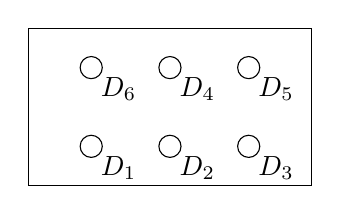
\begin{tikzpicture}[>=latex]
\draw(0.2,0.5) rectangle (4-.2,2.5);
\foreach \x in {1,2,3}
\foreach \y in {1,2}
{
    \draw(\x,\y)circle(4pt);
}
\node at (1,1)[below right]{$D_1$};
\node at (2,1)[below right]{$D_2$};
\node at (3,1)[below right]{$D_3$};
\node at (1,2)[below right]{$D_6$};
\node at (2,2)[below right]{$D_4$};
\node at (3,2)[below right]{$D_5$};

\end{tikzpicture}
    \caption{}
\end{figure}

演示这个实验最好用J2420型手摇三相交流发电机.实
验时将发电机输出端六个接线柱按星形接法接好,该机输出
端接线柱排列情况如图3.35所示,$D_1$、$D_2$、$D_3$分别为$A$、$B$、
$C$三相线圈的头,$D_4$、$D_5$、$D_6$分别为$A$、$B$、$C$三相线圈的尾,排
列成如图情况是为了便于进行星形连接与三角形连接。星形
接法只需将$D_6$、$D_4$、$D_5$端用铜片连在一起。用三个J0401型
演示电流表的检流计挡依次接在$D_1$、$D_2$、$D_3$与公共端(零线)
之间,并将三个表按$A$、$B$、$C$三相顺序放好,注意接线时电表
的三个负接线柱接零线。演示前在该机底板下电池盒内先装
入励磁用的四节干电池(6伏),演示时应先接通励磁开关,再
缓慢摇动手柄。注意不要使检流计超过满度电流,并尽可能使
转子转动周期与电表指针系统周期接近,这样可以明显演示
出三个电表指针依次摇动到右端。

\begin{figure}[htp]
    \centering
\includegraphics[scale=.7]{fig/3-36.png}
    \caption{}
\end{figure}

如果演示三相交流电的波形,最好让学生直接观察电网
中三相交流电的波形,实验电路如图3.36所示.示波器为
J2458型教学示波器,电子开关为J2460型教学用电子开关,
三个降压变压器可用三个学生实验用低压电源(J1202型)代
替,实验前需要确定相序。按图接好电路后,把示波器的Y
衰减拨至“10”,Y增益钮顺时针旋到底(最大增益),扫描频率
拨至“10—100”;使电子开关A增幅与B增幅钮反时针旋到
底(最小增益),开关频率拨至“5k—50k”挡;将三个变压器初
级线圈接入三相四线制电网。再调电子开关A增幅和示波器
扫描微调,使示波器荧光屏显示出两个周期的波形。调电子
开关B增幅与相对位移,使两个波形在屏上幅度相同,X轴重
合.然后观察B输出波形比A输出波形是否滞后$120^{\circ}$. 如
果不是,可将该变压器初级线圈接线颠倒一下。同理,再将电
子开关B输入端改接第三个变压器2伏输出端,调整后使其
波形滞后A$240^{\circ}$. 在确定好相序后,就可在课堂上进行演示
了。需要说明的是,经上述方法调整的相序可能不是电网原
来的相序。若想严格显示电网的相序,需要弄清三个变压器
初次级头尾,或者使用教学用三相变压器,如JYB-1型变
压器,由于电子开关只有两路,因而只能先后显示第一相与
第二相、第一相与第三相的波形,如想同时演示三相波形,
则需再用一台电子开关接在上述电子开关与示波器之间,接
法如图3.37所示.
\begin{figure}[htp]
    \centering
\includegraphics[scale=.7]{fig/3-37.png}
    \caption{}
\end{figure}

\subsubsection{星形接法与三角形接法的相电压与线电压}
按图3.38所示,制作电源接法示教板和负载接法示
教板。
\begin{figure}[htp]
    \centering
\includegraphics[scale=.7]{fig/3-38.png}
    \caption{}
\end{figure}

演示电源的两种接法时,可将J2420型手摇三相发电机
三组线圈按头尾顺序与图3.38中甲示教板相应接线柱相
接,或将演示实验16第二种方法所确定的三个变压器次级相
序与头尾接入甲示教板中(相应电压拨至6V挡).用J0401
型演示电表交流25伏挡分别测出各组线圈两端电压。再先后
按星形接法与三角形接法连接示教板上各接线柱,用伏特表
分别测试这两种情况下的相电压与线电压得出相应结论。
J2420型手摇三相发电机在手轮转速为120转/分时,空载每
相绕组电压在12伏左右.实验时,可请学生摇发电机,教师用
电压表进行测量演示。

\begin{figure}[htp]
    \centering
\includegraphics[scale=.7]{fig/3-39.png}
    \caption{}
\end{figure}

在演示三相四线制送电,负载星形接法相电压与线电压
关系及三相负载平衡时中性线中电流为零的实验时,可以将
4个6—8伏指示灯分别用较短的导线悬挂连接在图3.38所
示乙示教板相应接线柱上,并从甲示教板上接出三相四线制
电源,如图3.39所示,摇动发电机或接通电源时,可以看
到三相指示灯都亮了,只有串在中性线上的灯泡不亮,用
J0401型演示电表交流25伏挡分别测出各相相电压与线电
压,可以看出$U_{\text{线}}=\sqrt{3}U_{\text{相}}$的关系.由于三相负载平衡,在
除去串联在中性线上的小灯时,可以看出不影响三相负载用
电,说明中性线上此时电流为零,可以省去。如果中性线上
仍串联小灯,若除去其中任一相的负载灯泡,都可以看到串联
在中性线上的小灯发光,另两相上灯光减弱,表明负载不平衡
时中性线上电流不为零。如果接着再除去中性线上串联的小
灯,则相当于另两相小灯串联接在线电压之间,此时,用伏特
计可以测出每灯两端电压并与线电压值进行比较说明。

在进行负载作三角形连接演示实验时,可将三个小灯按
三角形接法接在示教板上,但如果仍使用6—8伏指示泡,注
意手摇发电机转速不要太高,三个变压器的电源应拨至4伏
挡,以免烧毁小灯。

\subsubsection{旋转磁场和感应电动机原理}

\begin{figure}[htp]\centering
    \begin{minipage}[t]{0.48\textwidth}
    \centering
\includegraphics[scale=.7]{fig/3-40.png}
    \caption{}
    \end{minipage}
    \begin{minipage}[t]{0.48\textwidth}
    \centering
\includegraphics[scale=.7]{fig/3-41.png}
    \caption{}
    \end{minipage}
    \end{figure}

演示这个实验可用J2421型三相电机原理演示器,如果
没有,自制也并不困难,装置主要由三部分组成,带支架的可
旋转的蹄形磁铁,互成$120^{\circ}$角的三相线圈及一指针式支架(附
小磁针和铝框)。蹄形磁铁可用教学用蹄形磁铁,但需制作一
夹具与轴连接,可参考图3.40所示装置.三组线圈均可用
直径0.3毫米左右的漆包线绕成(300—400匝),分别包上
红、黄、绿三色胶带或布带,互成$120^{\circ}$角安装在木底座上,
将其接成星形,三个头与底座接线柱相接,如图3.41所示.
可用长针固定在小木座上制成支架。小磁针可用教学用的
小磁针或自制;封闭金属框可以用薄铜片焊成:一边中央开
一小孔(略大于针直径),相对一边只需用圆头小钉冲出一小
槽(不要穿透铜片),使用时安放在支架上,如图3.42所示。

\begin{figure}[htp]\centering
    \begin{minipage}[t]{0.48\textwidth}
    \centering
\includegraphics[scale=.7]{fig/3-42.png}
    \caption{}
    \end{minipage}
    \begin{minipage}[t]{0.48\textwidth}
    \centering
\includegraphics[scale=.7]{fig/3-43.png}
    \caption{}
    \end{minipage}
    \end{figure}

演示分两个步骤进行。
(1)将小磁针支在支架上放在可旋转的磁铁中间,旋转
磁铁,将看到小磁针随之转动,表明了磁铁旋转产生旋转磁
场。然后将小磁针放在三相线圈中,利用手摇三相发电机或上
面介绍的通过三个变压器接入三相电网获得的低压三相交流
电给三组线圈通电,就可发现小磁针也旋转,电源也可采用如
图3.43所示裂相电源模拟三相交流电进行演示.图中$R$可
将10欧2安(J2354型)滑动变阻器调至最大值使用,$C$可将
两个470微法耐压25伏以上电 解电容器 负极与负极相接串
联后将两个正极接入电路,电源可使用J1201型或J1202型
低压电源的交流6伏输出,或者用一降压小变压器与以上
电路组装在一起使用。

(2)将金属闭合导体(即铜片线框)支于支架上,先后放
在可旋转磁铁和三相线圈中,旋转磁铁或通入三相电观察闭
合导体的旋转情况,分别加以讨论。实验时还可反向旋转磁铁
或任意更换三相电接入的两个线头位置,观察闭合导体与刚
才旋转方向相反的情况。

\subsection{学生实验}
\subsubsection{用示波器观察交流电的波形}
这个实验要进行电学重要仪器操作技能的训练。在实际
教学时,由于课本上对仪器的使用、有关实验内容都有较详细
的说明,教师不宜在课堂上再详细讲解,可要求学生自己阅
读,以培养学生独立学习新仪器使用方法的能力,还可以提出
一些问题以引导学生阅读和操作,下面几个问题可供教学时
参考:
\begin{enumerate}
\item 学生示波器(J2459型)面板上调节旋钮和开关可分
为三组,这三组分别控制什么?分别包括哪些旋钮和开关?各
起什么作用?Y衰减置于“$\infty$”时是什么意思?
\item 如果被观察的信号电压幅度估计为20伏,Y衰减应
置于哪个位置?为什么?
\item 如果被观察信号频率是200赫,想观察到两个完整
波形,扫描范围应置于哪个位置?为什么?调整扫描微调钮的
目的是什么?
\item 学生信号源(J2465型)可以输出哪几种频率的正弦
低频信号?输出信号幅度由什么调节?一般我们所说低频信号
是指哪一频率范围的信号?
\item 设计一个实验步骤,定量测出信号发生器500赫低
频输出最大时的正弦交流电电压的最大值和有效值。
\end{enumerate}

\subsubsection{用示器观察交流电的整流和滤波}
这个实验所用器材除J2459型学生示波器及学生用低压
电源(J1202型)外,所用元器件均可由J2467型(或J2467-1
型)学生电子实验箱取出使用,课本上图10-5所示实验元件
即为该型号电子实验箱中元件外形。但需注意此型号电子实
验箱中电解电容耐压只有10伏,因而实验时,最好将课本上
所说6伏交流电源改为4伏进行实验,以确保电容不被击穿。
如果没有该型号的电子实验箱,各元件也可自制:二极管用
2CP或2CZ型,电解电容可用耐压16伏、100微法(两个)与
10微法(一个)的,电阻可选用200欧及1千欧1/4瓦(或1/8
瓦)碳膜电阻,各元件都可焊接在宽2厘米长5厘米的铜箔
板上,铜箔板两端只保留1.5厘米长铜箔,中间部分可用刀刻
去。为便于接线,两端可直立焊接一段较粗的裸铜丝,导线系
用两端均带夹子的短塑料多股导线,元件板中央可用白漆画
出相应元件符号与正负极。

\begin{figure}[htp]
    \centering
\includegraphics[scale=.7]{fig/3-44.png}
    \caption{}
\end{figure}

为使实验取得较好效果,可将实验步骤作如下改变:
\begin{enumerate}
    \item 先按图3.44所示电路在白纸上画出电路图,并将元件放好,
用导线将元件连接起来。开启示波器,通过观察$A$、$B$两点输
入交流波形将示波器调好,使屏上出现3、4个完整稳定波形.再观察$A'$、$B$两点向半波整流波形,先后在$A$、$B$间接入10
微法与100微法电容器,观察电容滤波作用和不同电容的效
果。要求学生在坐标纸上记录上述观察到的电压波形,并进
行比较说明.
\item 再按课本上图10.4所示电路实验观察$A''$、
$B'$间电压波形.如果观察$C_1$、$C_2$与$R$数值变化对滤波效果
影响,则另需准备两个5微法16伏电解电容与20欧左右的
电阻,才能得到较显著的效果。
\end{enumerate}

在进行这个实验时,可能有的学生会提出不接负载时能
否观察相应波形问题,教师可以从串联电路特点出发,说明示
波器相当一个内阻极高(1兆欧以上)的电压表,不接负载时,
相当于二极管与电压表串联,此时电路正反向电阻相差不多,
因而正反向电流接近,看到波形将几乎仍为交流波形。(实际
上是二极管正向时,所加电压小于导通电压,对2CP管来说,
这个电压约为0.6伏,是由二极管此时内阻很大而引起的,
或者说是二极管的非线性特性造成的。)因而不接负载电阻
$R_f$是不能观察整流效果的。可实际观察一下,以加深理解。

\subsubsection{研究变压器的作用}
做这个实验,每一组需要一块交流电压表,一块交流电流
表,在学校实验室中,可用万用表交流10伏或25伏挡代替电
压表,可用J0414型500毫安交流电流表。如果没有该型号
交流电流表,可以用以下两种方法解决,一是将电路(初级或
次级电路)中串入一个1欧0.5瓦精密电阻(RJJ精密金属膜
电阻,误差$\pm 1\%$)作为示波器的取样电阻,通过示波器测量电
阻两端电压再换算为电流值。实验前需对示波器进行调整,使
示波器Y衰减为1、Y增益顺时针旋到底(增益最大)时屏上
Y轴上每一格相当50毫伏,实验时可将这个1欧取样电阻接
在示波器Y输入与地接线柱间并固定好,相当于一个电流表
串入电路,读出交流波形峰峰值$U_{PP}$, 按下式计算电流有效
值(Y衰减为1时):
\[I=\frac{U_{PP}}{2\sqrt{2}R}\approx 0.35U_{PP}{\rm mA}\]
或
\[I\approx 0.35\x 50\x Y_{PP}(\text{格数})=17.5Y_{PP}{\rm mA}\]
这个方
法虽然麻烦一些,但也使学生得到一个实际利用示波器作定
量测试的机会,对提高学生使用示波器能力是有好处的。

另一种方法是将学生所用直流安培表加以改装,改装方
法主要是在电表电路中接入两个2AP型晶体二极管,接法
如图3.45所示,由于各种直流安培计表头内阻与满度电
流不同,一般选满度电流小些的,如3毫安的表头.分流电阻
详细计算方法可参考有关书籍,并需实际与标准表校准。由于
二极管的非线性特性,刻度盘也是非线性的,一般可实测绘制
刻度盘。
\begin{figure}[htp]\centering
    \begin{minipage}[t]{0.48\textwidth}
    \centering
\includegraphics[scale=.7]{fig/3-45.png}
    \caption{}
    \end{minipage}
    \begin{minipage}[t]{0.48\textwidth}
    \centering
\includegraphics[scale=.7]{fig/3-46.png}
    \caption{}
    \end{minipage}
    \end{figure}

该实验所需其他仪器有J1202型学生电源,J2426型小
型变压器,J2354-1型10欧2安滑线变阻器(四个接头可当分
压器使用),2.5伏及6—8伏指示灯各两个(连同灯座),实验
电路如图3.46所示.实验按以下步骤进行:

(1)首先观察变压器结构,该变压器有三组线圈,分别标
有“I120T”,“II240T”、“III60T”,作降压变压器时,初级线圈
用“I120T”即120匝绕组,额定电压为4伏.次级线圈用“III60
T”即60匝绕组.作升压变压器时,初级线圈仍用“I120”绕组,
次级线圈用“II240T”即240匝绕组。

(2)按图3.46所示电路连接好实际电路,若进行升压实
验,小灯泡应用6—8伏的;若进行降压实验,小灯泡应用2.5
伏的。在接通电源之前,应将变阻器滑动端置于输出电压较
小位置,接通电路,逐渐滑动变阻器滑动端,使小电灯发光(不
要太亮)。

(3)用万用表交流10伏挡分别测出初次级电压(即$AB$
间与$CD$间电压),并作出记录.验证$U_1:U_2=n_1:n_2$.

(4)断开$A$点,串入电流表(或在输入端并有取样电阻的
示波器Y输入端),读出初级线圈电流值,而后接好$A$点,断
开$B$点,再串入电流表测出次级线圈电流值,作出记录,验证
$I_1:I_2=n_2:n_1$. 计算$U_1I_1$与$U_2I_2$值,求出变压器效率$n$.

(5)在次级电路小灯两端并联一个相同的小灯,重复步骤(3)与(4)。

(6)切断电源,将变压器从电路中取出,拆开铁心,装入
另一线圈,准备作降压(或升压)实验。在装铁心时,注意两点:
一是插铁心片时要交叉叠放,即一层按图3.47甲位置放,另
一层按图3.47乙位置放,二是在铁心快装满时,最后几片
铁心片的插入要十分小心,不要损坏线圈。可以先用小改锥
在一侧铁心片与线圈间插入一些,使铁心片靠里挤紧,再将最
后几片对正逐一插入,插一片,用改锥挤一次。同时,还可用
小木锤轻轻敲击铁片,使铁片对正插入。最后用木锤将铁片
敲击整齐,再装上外壳。

\begin{figure}[htp]
    \centering
    \begin{tikzpicture}[scale=.7]
\begin{scope}
    \draw(0,0) rectangle (4,4);
    \draw(0,3)-- (4,1);
    \draw[fill=white](.8,.5) rectangle (1.5,3.5);
    \draw[fill=white](2.5,.5) rectangle (3.2,3.5);
    \node at (2,-.5){奇数层};
    \node at (2,-1.5){甲};
\end{scope}
\begin{scope}[xshift=6cm]
    \draw(0,0) rectangle (4,4);
    \draw(0,1)-- (4,3);
    \draw[fill=white](.8,.5) rectangle (1.5,3.5);
    \draw[fill=white](2.5,.5) rectangle (3.2,3.5);
    \node at (2,-.5){偶数层};
    \node at (2,-1.5){乙};
\end{scope}
    \end{tikzpicture}
    \caption{}
\end{figure}

(7)重复(2)至(5)步骤,进行实验.

以上所设实验器材与实验步骤连同课本的问题可以根据
学校情况印发实验提纲发给学生阅读,并要求学生画好实验
记录表格再进行实验。如果时间允许,可在测电流时增加测空
载时电流这一项内容。

\subsection{课外实验活动}
\subsubsection{自制测电笔}

这个课外制作,需向学生简单说明测
电笔的工作原理,氖管是一种稀薄气体辉光放电管。在试电
笔中氖管两极间加60伏左右电压,即可引起氖气放电,发出
桔红色辉光,此时通过氖管的电流约几十微安,但两极电压
增大时,管中电流相应增大而且增长较快,试电笔中,电阻起
降压和限流作用,它的阻值可以通过以下方法估算出来:在测
试火线时,人体一端与地相接,另一端(手)通过氖管与电阻串
联接入火线,此时串联电路总电压为220伏,通过电流约几十
微安(人体安全电流1毫安以下),氖管两端压降为60伏左
右,因此降落在电阻器和人体电阻上的电压为160伏左右。
由欧姆定律估算出电阻器和人体电阻的总电阻约为几兆欧。
实际上人体电阻在几百千欧以下,因此,在试电笔使用过程
中,在人体上降落的电压是很小的,是安全的。只有给学生
讲清原理后,学生课外制作时才会懂得如何安全进行实验。

在具体进行这个小制作时,可以发动学生想办法把测电
笔制作得更实用一些,例如利用废旧圆珠笔或钢笔套进行制
作,不一定局限于课本上介绍的材料。测试笔与火线接触部分
长金属探针最好套上一段塑料管,以免与其他导体或人体接
触发生事故。

有些学生实验后可能提出这样的问题:为什么人体并没
有和大地直接接触(如穿着胶鞋、站在木凳上)试电笔也能
亮?这个问题可启发学生从人体与大地间是一个电容器,而测
试的又是交流电这一点上进行思考。

\section{习题解答}
\subsection{练习-}
\begin{enumerate}
    \item 有人说线圈平面转到中性面的瞬间,穿过线圈的磁通量最大,因而线圈中的感生电动势最大;线圈平面跟中性面垂直的瞬间,穿过线圈的磁通量为零,因而线圈中的感生电动势为零,这种说法对不对?为什么?


    \begin{solution}
        这种说法是错误的。根据法拉第电磁感应定律,感
        生电动势的大小与穿过闭合回路的磁通量变化率成正比,而
        与磁通量大小无关。当线圈平面转到中性面时,虽然磁通量
        最大,但磁通量变化率为零,线圈中感生电动势也为零;而当
        线圈平面转到与中性面垂直位置时,虽然磁通量为零,但磁
        通量变化率最大,因而线圈中感生电动势最大。
    \end{solution}
    
    \item 在课本图3.1所示的实验中,在不改变$B$、$\ell$和$v$的数值的情况下,你有什么办法来提高电动势的最大值?并说明所依据的原理.


    \begin{solution}
        可以通过增加线圈匝数来提高电动势的最大值。因
        为线圈在切割磁力线的过程中,每匝线圈的感生电动势都相
        同,$n$匝线圈是$n$个单匝线圈的串联,产生的感生电动势是单
        匝线圈的$n$倍。
    \end{solution}
    
    \item 在课本图3.1所示的实验中,设$AB$边的长度为20厘米,线圈的宽$AD$为10厘米,磁感应强度$B$为0.01特,线圈的转数为50转/秒,求电动势的最大值,如果从线圈平面转过中性面30$^\circ$角的瞬时开始计时,经过0.01秒时电动势的瞬时值是多大?


    \begin{solution}
        用$\ell$和$\ell'$分别表示$ab$和$ad$的长度。当线圈平面
        与中性面垂直时,电动势最大,这时的电动势
    \[\mathcal{E}_m=2B\ell v\]
    因为
\[v=\omega r=2\pi n\frac{\ell'}{2}\qquad \text{($n$为转速)}\]
所以
\[\mathcal{E}_m=2B\ell2\pi n\cdot \frac{\ell'}{2} \]
代入数值得
\[\mathcal{E}_m=2\x3.14\x50\x0.01\x20\x10^{-2}\x10\x10^{-2}=0.06{\rm V}\]
若从线圈平面转过中性面$30^{\circ}$角瞬时开始计时,那么该
交流电表达式
\[\begin{split}
   e&= \mathcal{E}_m \sin(\omega t+\phi_0)\\
   &=0.06\sin\left(2\pi \x50\x t+\frac{\pi}{6}\right)\\
   &=0.06\sin\left(100\pi  t+\frac{\pi}{6}\right)
\end{split}\]
因此经0.01秒时电动势瞬时值为
\[\begin{split}
    e &=0.06\sin\left(100\pi  0.01+\frac{\pi}{6}\right)\\
    &=0.06\sin\left(\pi +\frac{\pi}{6}\right)\\
    &=-0.06\sin\frac{\pi}{6}=-0.06\x \frac{1}{2}= -0.03{\rm V}
 \end{split}\]
    \end{solution}
    
    \item 画出$u=30\sin(\omega t+\pi/2)$伏的电压图象和$i=2\sin(\omega t-\pi/4)$安的电流图象,以$\omega t$为横轴.

    \begin{solution}
        所求图象如图3.48甲、乙所示.
\begin{figure}[htp]
    \centering
\begin{tikzpicture}[>=latex, scale=.7]
\begin{scope}
\draw[->](-2,0)--(7,0)node[right]{$\omega t$};
\draw[->](0,-4)--(0,4)node[right]{$u({\rm V})$};
\draw[very thick, domain=-pi/2:2*pi, samples=300]plot(\x,{3*cos(\x r)});
\foreach \x/\xtext in {0.5*pi/\frac{\pi}{2}, pi/\pi, 1.5*pi/\frac{3}{2}\pi, 2*pi/2\pi}
{
    \draw(\x,0)node[below]{$\xtext$}--(\x,.2);
}
\draw[dashed](0,3)node[left]{30}--(2*pi,3)--(2*pi,0);
\draw[dashed](0,-3)node[left]{$-30$}--(pi,-3)--(pi,0);
\node at (-.3,-.3){$0$};
\node at (pi,-5){甲};
\end{scope}
\begin{scope}[xshift=11cm]
    \draw[->](-2,0)--(8,0)node[right]{$\omega t$};
    \draw(0,3)node[left]{2}--(.2,3);
\draw[->](0,-4)--(0,4)node[right]{$i({\rm A})$};
\draw[very thick, domain=-pi/2:2.25*pi, samples=300]plot(\x,{3*sin(\x r -.25*pi r)});
\foreach \x/\xtext in {0.5*pi/\frac{\pi}{2}, pi/\pi}
{
    \draw(\x,0)node[below]{$\xtext$}--(\x,.2);
}
\foreach \x/\xtext in {1.5*pi/\frac{3}{2}\pi, 2*pi/2\pi}
{
    \draw(\x,0)--(\x,.2)node[above]{$\xtext$};
}
\draw[dashed](0,2.121)node[left]{$1.41$}--(pi,2.121)--(pi,0);
\draw[dashed] (.5*pi,2.121)--(.5*pi,0);
\draw[dashed](0,-3)node[left]{$-2$}--(1.75*pi,-3)--(1.75*pi,0);
\draw[dashed](0,-2.121)node[left]{$-1.41$}--(2*pi,-2.121)--(2*pi,0);
\draw[dashed](1.5*pi,-2.121)--(1.5*pi,0);
\node at (pi,-5){乙}; 
\node at (-.3,-.3){$0$};
\end{scope}
\end{tikzpicture}
    \caption{}
\end{figure}
    \end{solution}
    
    \item 课本图3.1是一个发电机模型,只能供课堂演示之用,如果你有兴趣,可约请几位同学,共同研究一下怎样在此模型的	
	基础上加以改进,设计一个小发电机,如果感到知识不足,可自学或查阅有关电工学的书籍.


    \begin{solution}
        说明:此题有关制作可参考前面实验指导部分有关
        内容。
    \end{solution}
\end{enumerate}

\subsection{练习二}
\begin{enumerate}
    \item 有一个电容器,能耐压250伏,是否能接在220伏的交流电路上?为什么?


    \begin{solution}
        耐压250伏的电容器不允许接在220伏的交流电路上.这是由于220伏交流电路上电压的最大值可达到有效值
        的$\sqrt{2}$倍,即
        \[U_m=\sqrt{2}U=\sqrt{2}\x220=310{\rm V}\]
        把耐压
        250伏的电容器接入这个电路就有击穿并引起短路的可能。
    \end{solution}
    
    \item 线圈转动的角速度$\omega$也叫角频率(或圆频率),试就课本图3.1导出角频率$\omega$跟周期$T$或频率$f$的关系式.


    \begin{solution}
        线圈从课本图3.1中甲图位量匀速转到乙图所示位
        置,转过角度为$\pi$, 经历时间为$T/2$, 故由角速度定义式可得
\[\omega=\frac{\theta}{t}=\frac{\pi}{T/2}=\frac{2\pi}{T}\]
又因$f=1/T$,所以
\[\omega=\frac{2\pi}{T}=2\pi f\]
    \end{solution}
    
    \item 已知:$u_1=220\sqrt{2}\sin(100\pi t+\pi /6)$伏,$u_2=380\sqrt{2}\sin(100\pi t+\pi /3)$伏,求这两个交流电压的最大值、有效值、周期、频率、角频率和初相.这两个电压哪个超前?相差是多大?


    \begin{solution}
        由题目可知,$U_{m_1}=220\sqrt{2}$伏,
        $U_{m_2}=380\sqrt{2}$伏。
\[        U_1=\frac{U_{m_1}}{\sqrt{2}}=220{\rm V},\qquad U_2=
 \frac{V_{m_2}}{\sqrt{2}}=380{\rm V}\]
    \[\omega_1=100\pi {\rm rad/s},\qquad \omega_2=100\pi {\rm rad/s}\]
\[f_1=\frac{\omega_1}{2\pi}=\frac{100\pi}{2\pi}=50{\rm Hz},\qquad f_2=\frac{\omega_2}{2\pi}=\frac{100\pi}{2\pi}=50{\rm Hz}\]
\[T_1=\frac{1}{f_1}=\frac{1}{50}=0.02{\rm s},\qquad T_2=\frac{1}{f_2}=\frac{1}{50}=0.02{\rm s}\]
\[\phi_1=\frac{\pi}{6},\qquad \phi_2=\frac{\pi}{3}\]
因$\phi_2>\phi_1$,所以$u_2$超前$u_1$, 相差
$$\Delta\phi=\frac{\pi}{6}-\frac{\pi}{3}=-\frac{\pi}{6}$$
即$u_2$超前$u_1$ $\pi/6$
    \end{solution}
    
    \item 有一正弦交流电,频率是50赫,有效值是5安,初相
    是$-\pi/2$.写出瞬时值的表达式,并画出图象.

    \begin{solution}
\[\begin{split}
    I_m&=\sqrt{2}I=\sqrt{2}\x 5=7.07{\rm A}\\
    \omega&=2\pi f=2\pi\x 50=100\pi {\rm rad/s}\\
    \phi_0&=-\frac{\pi}{2}
\end{split}\]
瞬时值表达式为
\[i=7.07\sin\left(100\pi t-\frac{\pi}{2}\right){\rm A}\]
其图象如3.49图。
    \end{solution}


\begin{figure}[htp]\centering
    \begin{minipage}[t]{0.48\textwidth}
    \centering
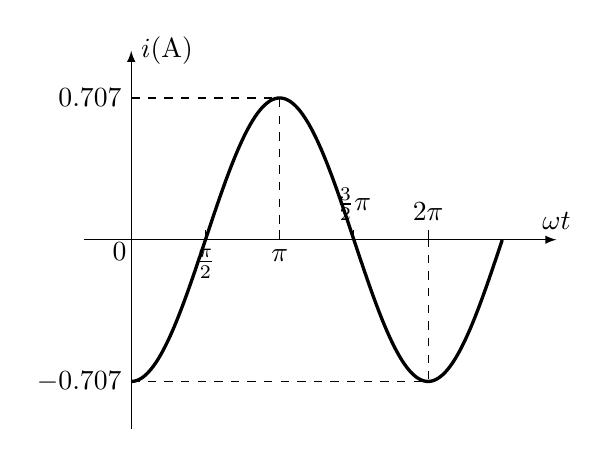
\begin{tikzpicture}[>=latex, scale=.6]
    \draw[->](-1,0)--(9,0)node[above]{$\omega t$};
\draw[->](0,-4)--(0,4)node[right]{$i({\rm A})$};
\draw[very thick, domain=0:2.5*pi, samples=300]plot(\x,{3*sin(\x r -.5*pi r)});
\foreach \x/\xtext in {0.5*pi/\frac{\pi}{2}, pi/\pi}
{
    \draw(\x,0)node[below]{$\xtext$}--(\x,.2);
}
\foreach \x/\xtext in {1.5*pi/\frac{3}{2}\pi, 2*pi/2\pi}
{
    \draw(\x,0)--(\x,.2)node[above]{$\xtext$};
}
\draw[dashed](0,-3)node[left]{$-0.707$}--(2*pi,-3)--(2*pi,0);
\draw[dashed](0,3)node[left]{$0.707$}--(pi,3)--(pi,0);
\node at (-.25,-.25){$0$};
    \end{tikzpicture}
    \caption{}
    \end{minipage}
    \begin{minipage}[t]{0.48\textwidth}
    \centering
    \begin{tikzpicture}[>=latex, yscale=1.4, xscale=.8]
       \draw [->](-.5,0)--(8.5,0)node[above]{$t$(s)};
    \draw [->](0,-1.5)--(0,2)node[right]{$i$(A)};
    \draw [ultra thick] plot[domain=0:3.14*2.5, samples=1000] function{cos(x)};
    \draw [dashed](0,1)--(2*3.1416,1);
    \draw [dashed](0,-1)--(3.1416,-1);
    \node at (0,1) [left]{$+10$};
    \node at (0,-1) [left]{$-10$};
    \foreach \x in {0.05,0.1,0.15,0.2,0.25}
    {
        \node at (\x*31.416, 0)[below]{$\x$};
        \draw(\x*31.416, 0)--(\x*31.416, .1);
    }
    \node at (-.25,-.25){$0$};
    \end{tikzpicture}
    \caption{}
    \end{minipage}
    \end{figure}

    \item 图3.50是某一正弦交流电的图象.根据图象求出最大值、有效值、周期、角频率和初相,并写出瞬时值的表达式.

    \begin{solution}
$I_m=10$安;$I=I_m/\sqrt{2}=0.707\x10=7.07$安;
$T=0.2$秒;

$\omega=\dfrac{2\pi}{T}=\dfrac{2\pi}{0.2}=10\pi{\rm rad/s}$;$\phi_0=-\dfrac{\pi}{2}$。

该交流电流瞬时值表达式为:
\[i=10\sin\left(10\pi t -\frac{\pi}{2}\right){\rm A}\]
    \end{solution}
    
    \item 课本图3.10是两个正弦交流电的图象,哪个超前,哪个落后?超前或落后的角度是多大?其中$\phi_1$和$\phi_2$的绝对值都是60$^\circ$.
    
\begin{solution}
$i_1$超前$i_2$ $120^{\circ}$, $i_2$落后$i_1$ $120^{\circ}$.
\end{solution}

\end{enumerate}


\subsection{练习三}
\begin{enumerate}
    \item 把“220V,40W”的灯泡接到照明电路中,通过灯泡的电流的最大值是多大?


    \begin{solution}
        因为$P=UI$, 所以在额定电压220V情况下,通过灯泡的电流有效值
 \[I=\frac{P}{U} =\frac{40}{220}=0.18{\rm A}\]
        因此电流的最大值
        $$I_m=\sqrt{2}\cdot I=\sqrt{2}\x0.18=0.25{\rm A}$$
    \end{solution}
    
    \item 在电阻$R$的两端加交变电压$u=220\sqrt{2}\sin(\omega t+\phi)$伏,$R=110$欧,写出电流瞬时值的表达式.


    \begin{solution}
    \[i=\frac{u}{R}=\frac{220\sqrt{2}}{110}\sin(\omega t+\phi)=2\sqrt{2}\sin(\omega t+\phi){\rm A}\]
    \end{solution}
    
    \item 在电阻为500欧的电阻丝中通以交流电,每秒钟产生5焦的热.求电流和电压的有效值和最大值,交流电的功率是多大?


    \begin{solution}
        由焦耳定律$\theta=I^2Rt$可得:交流电电流有效值
    \[I=\sqrt{\frac{\theta}{Rt}}=\sqrt{\frac{5}{500\x 1}}=0.1{\rm A}\]
电流最大值
\[i_m=\sqrt{2}I=0.14{\rm A}\]
        所以电压有效值
$$U=I\cdot R=0.1\x500=50{\rm V}$$
电压最大值
\[u_m=\sqrt{2}U=1.4\x50=70{\rm V}\]
交流电功率
\[P=\frac{W}{t}=\frac{5}{1}=5{\rm W}\]
    \end{solution}
    
    \item 把一个电热器接到10伏的直流电路中,每秒钟产生的热量为$Q$.现在把它改接到交流电路中,每秒钟产生的热量为$Q/2$,求交流电压的最大值.

    \begin{solution}
        对纯电阻电路而言,电路产生的热$$Q=\frac{U^2}{R}t$$
        接入直流电路时
        \[Q=\frac{U^2}{R}\x 1\]
        接入交流电路时
     \[\frac{Q}{2}=\frac{(U_m/\sqrt{2})^2}{R}t=\frac{U^2_m}{2R}\]
        两式相除可得:$U^2_m=U^2$, 
        所以
   \[     U_m=U=10{\rm V}\]
        即交流电压的最大值为10伏.
    \end{solution}
    
\end{enumerate}

\subsection{练习四}
\begin{enumerate}
    \item 一个线圈的自感系数为0.6亨,电阻只有几欧姆,把这个线圈接到50赫的交流电路中,它的感抗是多大?比较感抗和电阻的大小,说明为什么可以略去电阻,而认为它只有电感.


    \begin{solution}
        这个线圈对50赫交流电的感抗
    \[    X_L=2\pi fL=2\pi \x50\x0.6=188\Omega\]
        由于$X_L\gg R$, 因此在电路中起主要作用的是感抗而不是
        电阻,因而通常可以忽略电阻的作用而认为它只有电感。
    \end{solution}
    
    \item 有一个高频扼流圈,自感系数是25毫亨,对于1兆赫的交流电,它的感抗是多大?对于1千赫的交流电,它的感抗又是多大?


    \begin{solution}
        对1兆赫交流电的感抗
        \[X_{L_1}=2\pi f_1L=2\pi\x10^6\x25\x10^{-3}=157\x10^3\Omega\]
        对1千赫交流电的感抗
        \[X_{L_2}=2\pi f_2L=2\pi\x10^3\x25\x10^{-3}=157\Omega\]
    \end{solution}
    
    \item 一线圈的自感系数为0.5亨,电阻可以忽略.把它接到频率为50赫,电压为220伏的交流电路中,求通过线圈的电流.


    \begin{solution}
 \[I=\frac{U}{X_L}=\frac{U}{2\pi fL}=\frac{220}{2\x 3.14\x 50\x 0.5}=1.4{\rm A}\]   
    \end{solution}
    
    \item 有一线圈,电阻可略去不计.把它接到220伏、50赫的交流电路中,测得通过线圈的电流为2安.求线圈的自感系数.


    \begin{solution}
    因为\[I=\frac{U}{X_L}=\frac{U}{2\pi fL }\]
    所以
    \[L=\frac{U}{2\pi fI}=\frac{220}{2\pi\x 50\x 2}=0.35{\rm H}\]
    \end{solution}
    
\end{enumerate}


\subsection{练习五}
\begin{enumerate}
    \item 电容是100皮法的电容器,对频率是$10^8$赫的高频电流和频率是$10^3$赫的音频电流,容抗各是多大?


    \begin{solution}
对$10^6$赫高频电流,电容容抗
\[X_{C_1}=\frac{1}{2\pi f_1C}=\frac{1}{2\x3.14\x10^6\x100\x10^{-12}}=1.59\x10^3\Omega\]
对$10^3$赫音频电流,容抗
\[X_{C_2}=\frac{1}{2\pi f_2C}=\frac{1}{2\x3.14\x10^3\x100\x10^{-12}}=1.59\x10^6\Omega\]
    \end{solution}
    
    \item 把电容为5微法的电容器接到220伏、50赫的交流电路中,通过电容器的电流是多少?把电容器换为0.05微法的,通过的电流是多少?

    \begin{solution}
电容为5微法时,通过电容器的电流
\[\begin{split}
    I=\frac{U}{X_C}=\frac{U}{\dfrac{1}{2\pi fC}}&=U\cdot 2\pi fC\\
    &=220\x 2\pi\x 50\x 5\x 10^{-6}=0.345{\rm A}
\end{split}\]
当电容器电容为0.05微法时,通过电流
\[\begin{split}
    I'=\frac{U}{X'_C}=\frac{U}{\dfrac{1}{2\pi fC'}}&=U\cdot 2\pi fC'\\
    &=220\x 2\pi\x 50\x 0。05\x 10^{-6}\\
    &=3.45\x 10^{-3}{\rm A}=3.45{\rm mA}
\end{split}\]
    \end{solution}
    
    \item 在有220伏、50赫交流电源的地方,使用一个交流电流表可以测定电容器(耐压在311伏以上)的电容,说明测定的方法和原理.


    \begin{solution}
        根据$I=\dfrac{U}{X_C}$及$X_C=\frac{1}{2\pi fC}$可得:
\[        I=U\cdot 2\pi fC\]
        式中,$U$、$f$已知,$I$为通过电容器的电流,可用交流电流
        表测出,因而$C$可由下式求出:
        \[C=\frac{1}{2\pi f\cdot U}\]
    \end{solution}
    
    \item 线圈的自感系数为$L$,电容器的电容为$C$.要使感抗和容抗相等,交流电的频率应该满足什么条件?


    \begin{solution}
对同一电源要使线圈感抗和电容容抗相等,应满足
的关系是$X_L=X_C$, 即
\[2\pi fL=\frac{1}{2\pi fC}\]
因此电源频率应满足条件是
\[f^2=\frac{1}{4\pi^2 LC}\]
即
\[f=\frac{1}{2\pi\sqrt{LC}}\]
    \end{solution}
    
\end{enumerate}




\subsection{练习六}
\begin{enumerate}
    \item 变压器能不能改变直流电的电压?说明理由.


    \begin{solution}
变压器是利用交流电通过线圈在铁心中产生交变磁
通,从而使副线圈中引起感生电动势而完成变压作用的,对于
稳恒电流,由于不会引起磁通变化,也就无法完成变压作用。
因此,变压器不能改变直流电压。    
    \end{solution}
    
    \item 收音机中的变压器,原线圈有1210匝,接在220伏
的交流电源上,要得到5伏、6.3伏和350伏三种输出电压,
三个副线圈的匝数各是多少?


\begin{solution}
根据变压比公式可得
\[n_{\text{次}}=\frac{U_{\text{次}}}{U_{\text{初}}}\cdot n_{\text{初}}\]

5伏绕组匝数
\[n_1=\frac{U_1}{U_{\text{初}}}\cdot n_{\text{初}}=\frac{5}{220}\x 1210\approx 28\text{(匝)}\]
6.3伏绕组匝数
\[n_2=\frac{U_2}{U_{\text{初}}}\cdot n_{\text{初}}=\frac{6.3}{220}\x 1210\approx 35\text{(匝)}\]
350伏绕组匝数
\[n_3=\frac{U_3}{U_{\text{初}}}\cdot n_{\text{初}}=\frac{350}{220}\x 1210\approx 1925\text{(匝)}\]
\end{solution}

\item 为了安全,机床上照明电灯用的电压是36伏,这个
电压是把220伏的电压降压后得到的,变压器的原线圈是
1140匝,副线圈是多少匝?用这台变压器给40瓦的电灯供
电,原副线圈中的电流强度各是多大?


\begin{solution}
由变压比公式$\dfrac{U_1}{U_2}=\dfrac{n_1}{n_2}$,
可得副线圈匝数
\[n_2=\frac{U_2}{U_1}\cdot n_1=\frac{36}{220}\x 1140=187\text{(匝)}\]

当变压器副线圈向40瓦电灯供电时,通过副线圈的电流
\[I_2=\frac{P}{U}=\frac{40}{36}\approx 1.1{\rm A}\]
因为变压器的输出功率和输入功率相等,即$P_{\text{原}}=P_{\text{副}}=40$瓦,所以通过原线圈的电流
\[I_1=\frac{P_{\text{原}}}{U_{\text{原}}}=\frac{40}{220}=0.18{\rm A}\]
或:由$\dfrac{I_1}{I_2}=\dfrac{n_2}{n_1}$,可得:
\[I_1=\dfrac{n_2}{n_1}\cdot I_2=\frac{187}{1140}\x 1.1=0.18{\rm A}\]
\end{solution}

\item 利用变压器的原理可以测量线圈的匝数;用被测线
圈作原线圈,用一个匝数已知的线圈作副线圈,通入交流电,
测出两线圈的电压,就可以求出被测线圈的匝数,已知副线
圈有400匝,把原线圈接到220伏的线路中,测得副线圈的电
压是55伏,求原线圈的匝数.


\begin{solution}
    设原线圈匝数为$n_1$, 副线圈匝数为$n_2$, 原线圈电压
    为$U_1$, 副线圈电压为$U_2$. 根据变压比公式$\dfrac{U_1}{U_2}=\dfrac{n_1}{n_2}$,
    可得
\[n_1=\frac{U_1}{U_2}\cdot n_2=\frac{220}{55}\x 400=1600\text{(匝)}\]

\end{solution}

\item 在图3.28所示的电压互感器的电路中,为什么副线
圈的匝数比原线圈的少?在图3.29所示的电流互感器的电路
中,为什么副线圈的匝数比原线圈的多?


\begin{solution}
使用电压互感器是为了将被测的高电压转化成低电
压,根据变压器变压比公式可知,副线圈匝数要比原线圈少
得多。而使用电流互感器是为了将被测的强电流转化为弱电
流,根据变流比公式$I_1:I_2=n_2:n_1$可知,副线圈匝数比原线圈
多得多(事实上电流互感器的初级线圈只有一、二匝)。
\end{solution}

\end{enumerate}



\subsection{练习七}
\begin{enumerate}
    \item 在课文所给的例子中,用110伏和11千伏的电压输
电,分别要用96000${\rm mm}^2$和9.6${\rm mm}^2$的铝导线.如果不用铝
导线,而用铜导线,导线的横截面积分别要多大?

\begin{solution}
根据题意,导线的长度和电阻仍应与原来铝导线的
相同。根据电阻定律有:
\[R_{\text{铜}}=\rho_{\text{铜}}\cdot \frac{\ell_{\text{铜}}}{S_{\text{铜}}},\qquad R_{\text{铝}}=\rho_{\text{铝}}\cdot \frac{\ell_{\text{铝}}}{S_{\text{铝}}}\]
两式相除可得
\[\frac{S_{\text{铜}}}{S_{\text{铝}}}=\frac{\rho_{\text{铜}}}{\rho_{\text{铝}}}\]
所以,
\[S_{\text{铜}}=\frac{\rho_{\text{铜}}}{\rho_{\text{铝}}}\cdot S_{\text{铝}}\]
查课本第二册第180页电阻率表可知:
\[\rho_{\text{铜}}=1.7\x 10^{-8}\Omega\cdot {\rm m},\qquad   \rho_{\text{铝}}=2.9\x 10^{-8}\Omega\cdot {\rm m}\]

所以,用110伏输电时,使用铜导线截面积应为:
\[S_1=\frac{1.7\x 10^{-8}}{2.9\x 10^{-8}}\x 96000=56640{\rm mm^2}\]
用11千伏输电时,使用的铜导线截面积为:
\[S_2=\frac{1.7\x 10^{-8}}{2.9\x 10^{-8}}\x 9.6=5.7{\rm mm^2}\]
\end{solution}

\item 从发电站输出的功率为200千瓦,输电线的总电阻
为0.05欧,用110伏和11千伏的电压输电,在这两种情况
下,在输电线上损失的电压各是多少伏?输送到用户的电压各
是多少伏?在输电线上损失的功率各是多少千瓦?

\begin{solution}
输电线电阻与用户负载构成串联电路,电路消耗功
率为电站输出功率200千瓦.

因为$P=U\cdot I$, 所以$I=P/U$。
用110伏电压送电时,电路电流
\[I_1=\frac{200\x 10^3}{110}=1.82\x 10^3{\rm A}\]
用11千伏电压送电时,电路电流
\[I_2=\frac{200\x 10^3}{11\x 10^3}=18.2{\rm A}\]
\begin{enumerate}
    \item 用110伏电压送电时,输电线上损失电压
\[U_{\text{损}1}=I_1\cdot R=1.82\x10^3\x0.05=91{\rm V}\]
用户电压
\[U_{\text{用}1}=U_1-U_{\text{损}1}=110-91=19{\rm V}\]
输电线损失功率 
\[P_{\text{损}1}=I^2_1\cdot R=(1.82\x10^3)^2\x0.05{\rm W}=166{\rm kW}\]
\item 用11千伏电压送电时,输电线上损失电压
\[U_{\text{损}2}=I_2\cdot R=1.82\x 0.05=0.91{\rm V}\]
用户电压
\[U_{\text{用}2}=U_2-U_{\text{损}2}=11\x 10^3-0.91 {\rm V}\approx 11{\rm kV}\]
输电线损失功率 
\[P_{\text{损}2}=I^2_2\cdot R=1.82^2\x0.05{\rm W}\approx 0.017 {\rm kW}\]
\end{enumerate}
\end{solution}

\item 用220伏和11千伏两种电压来输电,输送的功率相
同,在输电线上损失的功率相同,导线的长度和电阻率也相
同,求导线的横截面积之比.

\begin{solution}
本题应根据损失功率列式进行比较。设输送端电压
为$U$, 输送功率为$P$, 导线电阻为$R$, 导线长度为$\ell$, 电阻率为
$\rho$、横截面积为$S$. 由输送电压与输送功率求出通过导线
电流:$I=P/U$。

由于导线上损失功率$P=I^2R$, 式中$R=\rho\cdot\dfrac{\ell}{S}$。
故损失功率可表示为
\[P=I^2R=\left(\frac{P}{U}\right)^2\cdot \rho\frac{\ell}{S}\]
若分别以220伏和11千伏输电,有
\[P_{\text{损1}}=\left(\frac{P}{U_1}\right)^2\cdot \rho\frac{\ell}{S_1},\qquad P_{\text{损2}}=\left(\frac{P}{U_2}\right)^2\cdot \rho\frac{\ell}{S_2}\]
因为$P_{\text{损1}}=P_{\text{损2}}$, 所以
\[\left(\frac{P}{U_1}\right)^2\cdot \rho\frac{\ell}{S_1}=\left(\frac{P}{U_2}\right)^2\cdot \rho\frac{\ell}{S_2}\]
整理后可得:
\[\frac{S_1}{S_2}=\frac{U^2_2}{U^2_1}=\frac{(11\x 10^3)^2}{220^2}=\frac{2.5\x 10^3}{1}\]
即:用220伏和11千伏输电两种情况导线横截面积之比
为$2.5\x10^3:1$.
\end{solution}

\end{enumerate}




\subsection{练习八}
\begin{enumerate}
	\item 图3.33中变压器副线圈$aO$间和$bO$间的交变电压都是6伏特.当$D_1$导通而$D_2$截止时,加在$D_2$上的反向电压的最大值是多大?

    \begin{solution}
设图3.51中的$O$点为零电势点.当变压器输出电
压处于正半周最大值时,$a$点电势为$+6\sqrt{2}$伏,$b$点电势为
$-6\sqrt{2}$伏,由于$D_1$处于正向电压作用而导通,$c$点和$a$点
电势接近相同,亦为$+6\sqrt{2}$伏.对二极管$D_2$而言,其正极
电势为$b$点电势为$-6\sqrt{2}$伏,而负极电势为$c$点电势$+6\sqrt{2}$伏,处于反向电压而截止,这个反向电压为$12\sqrt{2}\approx 17$伏($U_{cb}\approx 17$伏).因此加在$D_2$上反向电压最大值可达
17伏.
    \end{solution}

\begin{figure}[htp]\centering
    \begin{minipage}[t]{0.48\textwidth}
    \centering
\includegraphics[scale=.8]{fig/3-51.png}
    \caption{}
    \end{minipage}
    \begin{minipage}[t]{0.48\textwidth}
    \centering
\includegraphics[scale=.8]{fig/3-52.png}
    \caption{}
    \end{minipage}
    \end{figure}

	\item 课本图3.40是哪一种整流电路?试用带箭头的线画出当$a$正$b$负时电流的通路.

    \begin{solution}
        这是桥式整流电路,$a$正$b$负时电流通路如图3.52
        所示。
    \end{solution}
    
	\item 课本图3.41中的信号是正弦交流电,最大值为1伏,直流电源的电动势为4.5伏.画出负载$R$两端的电压波形,如果二极管$D$反接,负载$R$两端的电压又怎样?直流电源的内电阻略去不计.

\begin{solution}
    由于正弦交流电电压最大值为1伏,而电源电动势
为4.5伏,因此无论正弦交流信号处于正半周还是负半周,加
在二极管两端的电压始终是正向电压,处于导通状态。$R$两
端电压变化范围为3.5伏至5.5伏,$R$两端电压波形如图
3.53所示,如果二极管反接,则无论是交流信号的正半周还
是负半周,对二极管来说始终处于反向截止状态,通过$R$的电
流可认为是零,$R$两端电压也是零。
\begin{figure}[htp]
    \centering
\begin{tikzpicture}[>=latex, xscale=1, yscale=.6]
\draw[<->](0,7)node[right]{$u$(V)}--(0,0)--(8,0)node[right]{$t$};
\foreach \x in {0,1,2,...,6}
{
    \draw(0,\x)node[left]{\x}--(.1,\x);
}
\foreach \x in {4,5,6}
{
    \draw[dashed](0,\x)--(8,\x);
}
\draw[domain=0:2*pi+.3, samples=100, very thick] plot(\x, {sin(\x r)+5});

\foreach \x/\xtext in {1/\dfrac{T}{4},2/\dfrac{T}{2},3/\dfrac{3}{4}T,4/T}
{
    \draw(\x*pi/2,0)node[below]{$\xtext$}--(\x*pi/2,0.2);
}

\end{tikzpicture}
    \caption{}
\end{figure}
    \end{solution}
    
	\item 在课本图3.35所示的桥式整流电路中,如果二极管$D_1$的极性接反,会发生什么现象?如果二极管$D_1$已被击穿,又会发生什么现象?说明理由,并画出负载电阻上的电压波形.

    \begin{solution}
        二极管$D_1$极性接反电路如图3.54所示,当交流电
压处于正半周时,$a$正$b$负,由于$D_1$和$D_4$均处于反向电压
作用之下,各二极管与负载电阻$R$上都没有电流通过。而当
交流电压处于负半周时,即$a$负$b$正,此时$D_2$与$D_1$都处于正
向电压作用之下导通,造成$ab$两点短路,因而将造成$D_2$与
$D_1$因通过较大短路电流而烧毁,严重时将烧毁变压器,$R$上
也没有电流。


\begin{figure}[htp]\centering
    \begin{minipage}[t]{0.48\textwidth}
    \centering
\begin{circuitikz}[>=latex, scale=1]

        \draw (-3,.25)--(-3,1)--(-2,1) to [american inductor] (-2,-1)--(-3,-1)--(-3,-.25);
        \draw (1,-1)--(1,-1.5)--(-1.25,-1.5) to [american inductor] (-1.25,1.5)--(1,1.5)--(1,1);
        \draw [ultra thick] (-1.6, -.5)--(-1.6, .5);
      \ctikzset{diodes/scale=0.6}  
      \draw (0,0) to [full diode] (1,1) ;
      \draw (2,0) to [full diode] (1,1) ;
     \ctikzset{diodes/scale=0.6}  \draw (0,0) to [full diode] (1,-1) to [full diode] (2,0) ;
        \draw (2,0)--(2.5,0) to [european, R=$R$] (2.5,-2) --(-.5,-2)--(-0.5,0)--(0,0);
        
        \draw [fill=white] (-3,.25) circle (1pt);
        \draw [fill=white] (-3,-.25) circle (1pt);
        \draw [fill=black] (0,0) circle (1pt);
        \draw [fill=black] (2,0) circle (1pt);\draw [fill=black] (1,-1) circle (1pt);
        \draw [fill=black] (1,1) circle (1pt);
        \node at (-3,0){$\sim $};
        \node at (1.5,1){$D_1$};        \node at (1.5,-1){$D_2$};
        \node at (.5,-1){$D_3$};        \node at (.5,1){$D_4$};
        \node at (-1.1,.5){$a$};        \node at (-1.1,-.5){$b$};
        \end{circuitikz}

    \caption{}
    \end{minipage}
    \begin{minipage}[t]{0.48\textwidth}
    \centering
\begin{tikzpicture}[>=latex, xscale=1, yscale=1.2]
\draw[<->](0,1.7)node[right]{$U_R$}--(0,0)--(5.75,0)node[right]{$t$};
\draw(0,0)--(0,-1);
\foreach \y in {0,2,4}
{
    \draw[domain=0:1, samples=50, very thick] plot(\x+\y, {sin(\x*pi r)});
}
\foreach \x/\xtext in {1/\dfrac{T}{2},2/T,3/\dfrac{3}{2}T,4/2T,5/\dfrac{5}{2}T}
{
    \draw(\x,0)node[below]{$\xtext$}--(\x,0.1);
}
\draw(0,1)node[left]{$U_m$}--(.1,1);
\end{tikzpicture}
    \caption{}
    \end{minipage}
    \end{figure}

如果$D_1$被击穿,相当于$D_1$被短路.在交流电正半周,即
$a$正$b$负时,$R$上将有电流通过。而当交流电负半周,即$a$负$b$
正时,$D_2$处于正向导通,直接将$ab$两点短路.$R$因两端电势相
同,而没有电流通过.因此仍将出现烧毁$D_2$现象,并有烧毁
变压器可能.负载$R$上的电压波形如图3.55所示。
    \end{solution}
\end{enumerate}


\subsection{练习九}
\begin{enumerate}
    \item 根据课本图3.49写出三相负载相同时的相电流的瞬时值的表达式,并利用数学中学过的三角知识证明:三个相电流之和在任何时刻都等于零.

    \begin{proof}
        相电流的瞬时值表达式分别为
        \[\begin{split}
        i_a&=I_m\sin \omega t\\
        i_b&=I_m\sin(\omega t-120^{\circ})\\
        i_c&=I_m\sin(\omega t-240^{\circ})        
        \end{split}\]
        三个相电流之和
       \[ i_a+i_b+i_c=I_m\sin \omega t+I_m\sin(\omega t-120^{\circ})+I_m\sin(\omega t-240^{\circ})  \]
        根据三角函数和差化积公式
\[\sin A+\sin B=2\sin\frac{A+B}{2}\cdot\cos\frac{A-B}{2}\]
        可得:
\[\begin{split}
    i_a+i_b+i_c&=I_m\sin \omega t+I_m\left[\sin(\omega t-120^{\circ})+\sin(\omega t-240^{\circ}) \right]\\
    &=I_m\sin \omega t+2I_m\sin\frac{(\omega t-120^{\circ})+(\omega t-240^{\circ})}{2}\cdot \cos\frac{(\omega t-120^{\circ})-(\omega t-240^{\circ})}{2}\\
    &=I_m\sin \omega t+2I_m\cdot \sin(\omega t-180^{\circ})\cdot \cos 60^{\circ}\\
    &=I_m\sin \omega t+2I_m\cdot (-\sin \omega t)\cdot \frac{1}{2}\\
    &=I_m\sin \omega t - I_m\sin\omega t=0 
\end{split}\]
    \end{proof}
    
    \item 在课本图3.46所示的三相四线制电路中,相电压是220伏.现有“220V,100W”的灯泡90盏,第一相安装40盏,第二相安装30盏,第三相安装20盏.求灯泡全接通时,各个相电流和线电流.

    \begin{solution}
        在三相四线制电路中,相电流和线电流相同。
        因此,第一相电流
\[I_{\text{相1}}=I_{\text{线1}}=\frac{P}{U}\cdot n_1=\frac{100}{220}\x 40=18.2{\rm A}\]
第二相电流
\[I_{\text{相2}}=I_{\text{线2}}=\frac{P}{U}\cdot n_2=\frac{100}{220}\x 30=13.6{\rm A}\]
第三相电流
\[I_{\text{相3}}=I_{\text{线3}}=\frac{P}{U}\cdot n_3=\frac{100}{220}\x 20=9.1{\rm A}\]
    \end{solution}
    
    \item 如果电源采用课本图3.53所示的三角形连接,线电压和相电压的关系是怎样的?设各相线圈的情况相同.

    \begin{solution}
这种情况下两根端线间电压和直接与这两端线相连
的那一相电压相同(图3.56甲).即线电压和相电压相同.
\begin{figure}[htp]\centering
    \begin{circuitikz}[scale=1.2]
\begin{scope}
    \draw (0,0) to [american inductors, L=3] (-1.5, -2);
        \draw (0,0) to [american inductors, L=1] (1.5, -2);	
            \draw (1.5, -2) to [american inductors, L=2] (-1.5, -2);
        \draw (0,0)-- (2.5,0)node [right]{$A$};
        \draw (1.5, -2)-- (2.5,-2)node [right]{$B$};	
        \draw (-1.5, -2)--(-1.5, -3)-- (2.5,-3)node [right]{$C$};	
        \foreach \x in {-2,-3,0}
        {
            \draw[fill=white] (2.5,\x) circle({1.5pt});
        }
        \draw [fill=black](0,0) circle(1.5pt);
        \draw [fill=black](1.5, -2) circle(1.5pt);
        \draw [fill=black](-1.5, -2) circle(1.5pt);
        \node at (0.5,-3.5){甲};
\node at (0,0)[above left]{尾};
\node at (0,0)[below right]{头};
\node at (-1.5, -2)[above left]{头};
\node at (-1.5, -2)[below right]{尾};
\node at (1.5, -2)[above right]{尾};
\node at (1.5, -2)[below left]{头};

\end{scope}
       \begin{scope}[xshift=6cm]
    \draw (0,0) to [american inductors, L=3] (-1.5, -2);

        \draw (1.5,-.25)node[right]{$A'$}--(.25,-.25) to [american inductors, L=1] (1.25, -1.75)--(2,-1.75)node[right]{$B'$};	


            \draw (1.5, -2) to [american inductors, L=2] (-1.5, -2);
        \draw (0,0)-- (2.5,0)node [right]{$A$};
        \draw (1.5, -2)-- (2.5,-2)node [right]{$B$};	
        \draw (-1.5, -2)--(-1.5, -3)-- (2.5,-3)node [right]{$C$};	
        \foreach \x in {-2,-3,0}
        {
            \draw[fill=white] (2.5,\x) circle({1.5pt});
        }

        \node at (0.5,-3.5){乙};

        \node at (0,0)[above left]{尾};
        \node at (.25,-.25)[below]{头};
        \node at (-1.5, -2)[above left]{头};
        \node at (-1.5, -2)[below right]{尾};
        \node at (1.25, -1.75)[above right]{尾};
        \node at (1.5, -2)[below left]{头};

        \draw[fill=white] (1.5,-.25) circle({1.5pt});
        \draw[fill=white] (2,-1.75) circle({1.5pt});
\end{scope} 
    \end{circuitikz}
    \caption{}
    \end{figure}


说明:能否这样连接取决于能否证明任一时刻$u_{AB}=u_{AC}+u_{CB}$。
实际上三角形连接是将各相线圈头尾相接的,
为证明方便,我们先假定将第一相头尾与电路脱离开。如
图3.56乙所示,那么

第一相头尾电压瞬时值为:$u_{AB}=U_m\sin\omega t$.

第二相与第三相头尾相接后$BA$两点电压(注意顺序)瞬
时值为:
\[\begin{split}
    u_{BA}&=u_{BC}+u_{CA}\\
&=U_m\sin (\omega t-120^{\circ})+U_m\sin (\omega t-240^{\circ})\\
&=U_m[\sin (\omega t-120^{\circ})+\sin (\omega t-240^{\circ})]\\
&=U_m\cdot 2\sin(\omega t-180^{\circ})\cdot \cos 60^{\circ}\\
&=U_m\cdot 2\cdot (-\sin\omega t)\cdot \frac{1}{2}\\
&=-U_m\sin\omega t
\end{split}\]
\[u_{AB}=-u_{BA}=U_m\sin\omega t=U_{A'B'}\]
上式表明$AB$两点电压变化与$A'B'$两点电压变化是完全
相同的,即任一时刻$AB$两点电压与$A'B'$两点电压相同,因
此可以将$A$与$A'$点相接,$B$与$B'$相接而形成电源的三角形
连接。
    \end{solution}
    
\end{enumerate}



\subsection{练习十}
\begin{enumerate}
    \item 有一台感应电动机,铭牌上标有“220/380”“$\triangle$/Y”的字祥.这表示这台电动机每相定于线圈的额定电压是 220伏,如果线电压是220伏,定子线圈要连成三角形;如果线电压是380伏,定子线圈要连成星形,为什么?


    \begin{solution}
当定子线圈接成三角形时,加在每相定子线圈上的
电压与供电电路的线电压相同,所以供电电路的线电压为
220伏时,加在每相线圈上的电压也是220伏,就可使电机正
常运转.如果供电电路的线电压是380伏,就需要把电动机定
子线圈连成星形。这是因为,星形连接时,每相线圈的电压与
供电电路线电压关系为$U_{\text{线}}=\sqrt{3}U_{\text{相}}$. 所以$U_{\text{相}}=380/\sqrt{3}=220$伏,才可使电机正常运转.
    \end{solution}
    
    \item 实验表明:只要把定子上任意两组线圈的电流互换一下,旋转磁场就向相反方向旋转.画出类似于课本图3.56的
    图,并加以分析说明.


    \begin{solution}
    课本图3.56中,$AX$绕组通以$i_{AX}$, $BY$通以$i_{BY}$,
$CZ$通以$i_{CZ}$. 那么产生磁场将沿逆时针方向旋转。现在,将
某两个组定子绕组中通过的电流互换,例如将$BY$绕组中通
以$i_{CZ}$电流,而$CZ$绕组中通以$i_{BY}$电流,则其旋转磁场情况
如下:
\begin{itemize}
\item 在$t=0$时刻,$AX$中电流为零;$BY$中电流$i_{CZ}$, 由$B$端流
入、$Y$端流出;$CZ$中电流$i_{BY}$, 由$Z$端流入、$C$端流出。合成
磁场方向如图3.57甲中虚线所示,其方向指向$X$.

\item 在$t=T/3$时刻,$CZ$中电流为$i_{BY}=0$; $AX$中电流$i_{AX}$, 
由$A$端流入、$X$端流出;$BY$中电流$i_{CZ}$由$Y$端流入、$B$端流
出,合成磁场方向如图3.57乙中虚线所示,其方向指向$Z$.
\end{itemize}

显然经过$T/3$, 合成磁场方向指向沿顺时 针方向由$X$移
至$Z$, 转过$120^{\circ}$. 图3.57丙和丁中虚线分别表示在$2T/3$及$T$
时刻合成磁场情况,可以看出经过一个周期$T$, 合成磁场也相
应沿顺时针方向转过一圈。因此任意对调两个绕组中的电流,
就可使旋转磁场方向改变转向。
\begin{figure}[htp]
    \centering
    \includegraphics[scale=.7]{fig/3-57.png}
    \caption{}
\end{figure}
    \end{solution}
    
    \item 在课本图3.54所示的实验中,铝框总要比磁铁转得慢,即比旋转磁场转得慢,而不能跟磁场转得一样快,即不能同步旋转,因此感应电动机也叫异步电动机,试说明铝框为什么不能跟磁铁同步旋转.

    \begin{solution}
使铝框转动的旋转力矩,是由于在铝框中产生的感
生电流受到磁场力而引起的。因此,铝框与磁铁间有相对运
动而发生切割磁力线现象是铝框转动的前提。如果某一瞬间
铝框与旋转磁场同步转动,那么,铝框就不切割磁力线,感生
电流也就消失了,所受磁场力矩随之消失。在阻力矩作用下,
铝框转速会减小,铝框转速减小了,又会切割磁力线产生感
生电流,且随着转速减小,电流逐步增大,铝框所受磁场力矩
也将增大,直至转速减小到一定程度,使电磁力矩和阻力矩平
衡,而使铝框维持匀速转动为止。这就是铝框转速永远小于
磁场转速,不能同步旋转的道理。 
    \end{solution}
    
\end{enumerate}




\subsection{习题}
\begin{enumerate}
    \item 把电阻和电容器串联在交流电路中,测得电阻上的电压为30伏,电容器上的电压为40伏.已知电阻的阻值为200欧,交流电的频率为50赫,求电容器的电容,这道题提供了一种用伏特表测定电容的方法.


    \begin{solution}
在交流电路中,任一瞬间通过串联电路各处的电流
都是相同的。电路中电流的有效值为
\[I=\dfrac{U_R}{R}=\frac{30}{200}=0.15{\rm A}\]
对于电容器部分,可以看成一个纯电容电路,因而有:
\[I=\frac{U_C}{X_C}=\frac{U_C}{\dfrac{1}{2\pi fC}}=U_C\cdot 2\pi fC\]
\[C=\frac{I}{U_C\cdot 2\pi f}=\frac{0.15}{40\x 2\pi\x 50}=12\x ^{-6}{\rm F}=12{\rm mF}\]
    \end{solution}
    
    \item 把电阻和电容器并联在交流电路中,已知电阻的阻值是500欧,电容器的电容是30微法.当交流电的频率为50赫时,通过电阻和电容器的电流之比是多大?当交流电的频率是500赫时,电流之比又是多大?


    \begin{solution}
在交流电路中,并联各支路两端电压在任一瞬间都
是相同的,因此设电阻与电容器两端电压为$U$. 因为
\[I_R=\frac{U}{R},\qquad I_C=U\cdot 2\pi fC\]
所以
\[\frac{I_R}{I_C}=\frac{U/R}{U\cdot 2\pi fC}=\frac{1}{R\cdot 2\pi fC}\]
当电源频率为50赫时
\[\frac{I_R}{I_C}=\frac{1}{R\cdot 2\pi fC}=\frac{1}{500\x 2\pi\x 50\x 30\x 10^{-6}}\approx 0.21\]
当电源频率为500赫时
\[\frac{I_R}{I_C}=\frac{1}{R\cdot 2\pi fC}=\frac{1}{500\x 2\pi\x 500\x 30\x 10^{-6}}\approx 0.021\]
    \end{solution}
    
    \item 变压器的原线圈为1100匝,副线圈为180匝,原线圈接到220伏的交流电路中,副线圈上并联了3个阻值都是90欧的用电器.如果原线圈允许通过的最大电流为0.9安,副线圈上最多还可以并联多少个阻值为60欧的用电器?


    \begin{solution}
根据变压比公式$\dfrac{U_1}{U_2}=\dfrac{n_1}{n_2}$
可得:
副线圈电压
\[U_2=\frac{n_2}{n_1}\cdot U_1=\frac{180}{1100}\x220=36{\rm V}\]
根据变流比公式$\dfrac{I_1}{I_2}=\dfrac{n_2}{n_1}$
可得:
副线圈允许通过的最大电流为
\[I_2=\frac{n_1}{n_2}\cdot I_1=\frac{1100}{180}\x 0.9=5.5{\rm A}\]
3个90欧的用电器并联在副线圈上,副线圈上通过的
电流为:
\[I=\frac{U_2}{R_{\text{并}}}=\frac{36}{90/3}=1.2{\rm A}\]
副线圈还可增加负载电流 
\[I'=I_2-I=5.5-1.2=4.3{\rm A}\]
设还可并联$m$个60欧用电器,其总电流不超过4.3安.即
\[m\cdot\frac{U_2}{60\Omega}\le I'\]
所以
\[m\cdot \frac{36}{60}{\rm A}\le 4.3{\rm A}\]
即:$m\le 7.17$.

因此,最多还可并联7个60欧的用电器.
    \end{solution}
    
    \item 有一个教学用的可拆变压器,它的原副线圈外部还可绕线,现在要测定原副线圈的匝数.现有一根足够长的绝缘导线,还需要什么器材?简要说明实验原理.

    \begin{solution}
还需一块能测较高电压的交流电压表和一块可测几
伏特的小量程电压表,将绝缘导线在副线圈(或原线圈)外部
绕几十匝,将变压器重新组装好后,按原线圈规定电压接入电
源,分别实测原线圈两端、副线圈两端和加绕线圈两端电压
值,根据变压比公式就可以计算出原副线圈匝数。

由$\dfrac{U_1}{U_2}=\dfrac{n_1}{n_2}$可得$n_1=\dfrac{U_1}{U_2}\cdot n_2$. 其中$U_1$、$U_2$可实测,$n_2$
为加绕线圈匝数,便可求出原副线圈匝数。

注意:实际上进行这个实验时,需要根据所给变压器的
-具体情况和要求测量的准确程度进行测量,所用伏特计一般
采用多量程的,如万用表交流电压挡。实验电源也可以用低
压电源,将低电压加在加绕线圈上进行测量,如果仅有一块
单量程较高电压的电压表,也可以用如下方法测量:

将加绕线圈与原线圈(或副线圈)串联起来。测出原线圈
两端电压和串联绕组总电压,由下式求出原线圈匝数。
\[\frac{U_{\text{原}}}{U_{\text{总}}-U_{\text{原}}}=\frac{n_{\text{原}}}{n_{\text{加}}}\]
    \end{solution}
    
    \item 课本图3.59是电工常用的钳形电流表,可以用来测定交变电流,把钳口打开,把被测的通电导线放在钳口中间(右图),交流电表就可以测出导线中的电流强度.试说明钳形电流表的工作原理.

\begin{solution}
    钳形电流表实际上是一种电流互感器,用以测定强
    交流电电流。当导线中有交变电流通过时,在环绕导线的铁
    心中有变化磁通,从而使绕在铁心上的线圈产生感生电流,接
    在绕组两端的电流表即可读出读数。通电导线中电流越大,
    在铁心中磁通变化率就越大,感生电流也就越大,电流表的读
    数相应就越大,这就是钳形电流表的工作原理。
\end{solution}

    \item 在课本图3.35所示的桥式整流电路中,变压器原副线圈的匝数比等于8,原线圈接在220伏的交流电路中,能不能选用最高反向工作电压为50伏的晶体二极管进行整流?为什么?

\begin{solution}
    副线圈两端电压
    \[U_{\text{副}}=\frac{n_{\text{副}}}{n_{\text{原}}} \cdot U_{\text{原}}= \frac{1}{8}\x220=27.5{\rm V}\]
在课本图3.35所示桥式整流电路中,每个二极管承受的反向
电压可从面分析得知:

在交流电压正半周时,$D_1$与$D_3$导通,这两个二极管两端
电势可认为相同(忽略二极管自身压降),而$D_2$与$D_4$反向截
止,相当于跨接在$a,b$两点间,因而其反向承受最大电压为
变压器次级电压最大值.同理可知$D_1$与$D_4$情况,即
\[U_{km}=U_m=\sqrt{2}\cdot U_{\text{副}}=\sqrt{2}\x27.5=38.9{\rm V}<50{\rm V}\]
因此可以选
用最高反向工作电压为50伏的晶体二极管进行整流。
    \end{solution}
    
    \item 课本图3.60是电子技术中用到的限幅电路,电池组的电动势都为$\mathcal{E}$,左端输入的是正弦交流电,电压$u_1$的最大值为$2\mathcal{E}$.试画出右端输出的电压$u_2$的图象,并分析说明理由.电池组的内电阻略去不计.

\begin{solution}
右端输出电压$u_2$的图象如图3.58乙所示.图甲表
示输入端$u_1$的图象。

\begin{figure}[htp]
    \centering
\begin{tikzpicture}[>=latex, xscale=1.7, yscale=1.3]
\begin{scope}
    \draw[->](0,-1.5)--(0,1.5)node[right]{$u_1$};
    \draw[->](0,0)node[left]{0}--(3.5,0)node[right]{$t$};
\draw[very thick, domain=0:3, samples=500] plot(\x,{sin(\x*pi r)});
\draw[dashed](0,1)node[left]{$2\mathcal{E}$}--(2.8,1);
\draw[dashed](0,-1)node[left]{$-2\mathcal{E}$}--(1.8,-1);
\node at (1.5,-1.5){甲};
\draw(0,-.5)node[left]{$-\mathcal{E}$}--(.1,-.5);
\draw(0,.5)node[left]{$\mathcal{E}$}--(.1,.5);
\node at (1,0)[below left]{$\dfrac{T}{2}$};\node at (2,0)[below right]{$T$};
\end{scope}
\begin{scope}[xshift=4.5cm]
    \draw[->](0,-1.5)--(0,1.5)node[right]{$u_2$};
    \draw[->](0,0)node[left]{0}--(3.5,0)node[right]{$t$};
\draw[very thick, domain=0:1/6, samples=50] plot(\x,{sin(\x*pi r)});
\draw[very thick](1/6,.5)--(5/6,.5);
\draw[very thick, domain=5/6:7/6, samples=50] plot(\x,{sin(\x*pi r)});
\draw[very thick](7/6,-.5)--(11/6,-.5);
\draw[very thick, domain=11/6:13/6, samples=50] plot(\x,{sin(\x*pi r)});
\draw[very thick](13/6,.5)--(17/6,.5);
\draw[very thick, domain=17/6:3, samples=50] plot(\x,{sin(\x*pi r)});
\node at (1,0)[below left]{$\dfrac{T}{2}$};\node at (2,0)[below right]{$T$};
\draw[dashed](0,.5)node[left]{$\mathcal{E}$}--(2.8,.5);
\draw[dashed](0,-.5)node[left]{$-\mathcal{E}$}--(1.8,-.5);
\draw(0,-1)node[left]{$-2\mathcal{E}$}--(.1,-1);
\draw(0,1)node[left]{$2\mathcal{E}$}--(.1,1);
\node at (1.5,-1.5){乙};
\end{scope}
\end{tikzpicture}
    \caption{}
\end{figure}

当$u_1$处于正半周时,如果$u_1<\mathcal{E}$, 对$D_2$所在支路来说,由
于$D_2$始终处于反向电压作用,因此$D_2$截止,该支路被视为断
路状态,对于$D_1$所在支路来说,由于$D_1$正极电势仍低于负极
电势,因而也处于截止状态,所在支路也可视为断路状态,因
此$R$上几乎没有压降,$u_2$与$u_1$电压变化相同.如果$u_1$增大
至$u_1>\mathcal{E}$, $D_2$仍然受反向电压的作用,$D_2$所在支路仍可视为断
路状态,而对$D_1$所在支路,由于$D_1$正极电势大于负极电势,
$D_1$导通.$R$两端电压为$u_1-\mathcal{E}$, $R$中有电流通过.而输出端电
压由于电池组作用而基本维持与电动势$\mathcal{E}$相同。换言之,当
正半周$u_1<\mathcal{E}$时,输出与输入相同,当$u_1>\mathcal{E}$时,输出端电压
维持$\mathcal{E}$不变,从而起到限幅作用,同理可分析负半周情况。
\end{solution}

    \item 在课本图3.46所示的三相四线制照明电路中,设$A$相接通了8盏“220V,100W”的灯泡,$B$相接通了2盏“220V,100W”的灯泡,$C$相中没有接通灯泡,这时接通的灯泡都正常发光,因某种原因中性线断开了(在该图中$O$处断开),将会发生什么现象?说明理由.
 
    \begin{solution}
如果中性线断开,$A$相与$B$相灯泡串联起来,串联
电路两端电压将是线电压380伏,由于两组灯泡是串联,其电
阻之比为
\[R_A:R_B=\frac{R}{8}:\frac{R}{2}=1:4\]
式中$R$表示每一灯泡电阻,因而这两组灯泡电压分配之比
\[U_A:U_B=R_A:R_B=1:4\]
所以$A$相灯泡两端电压为\[U_A=\frac{1}{5}\x 380=76{\rm V}\]
$B$相灯泡两端电压为\[U_B=\frac{4}{5}\x 380=304{\rm V}\]
因此,$B$相灯泡将因电压过高而烧毁。

由此可见,在三相四线制供电电路中,中性线在任何情
况下不允许断开,以免造成用电器因电压变高而烧毁的现象
发生。这也是中性线不允许安装开关和保险丝的原因。
    \end{solution}
    
    \item 如课本图3.61所示,电源采用星形连接,负载采用三角形连接.电源的相电压是220伏,各相负载相同,阻值都是110欧,求通过各相负载的相电流和线电流.

\begin{solution}
    电源部分的线电压
   \[ U_{\text{线}}=\sqrt{3}U_{\text{相}}=\sqrt{3}\x220=380{\rm V}\]
   负载电路是三角形连接,其相电压与线电压相同,
\[  U'_{\text{相}}=U'_{\text{线}}=220\sqrt{3}=380{\rm V}\]
   负载相电流
   \[I_{\text{相}}=\frac{U'_{\text{相}}}{R}=\frac{220\sqrt{3}}{110}=3.46{\rm A}\]
   负载线电流 
\[I_{\text{线}}=\sqrt{3} I_{\text{相}}=\sqrt{3}\x\frac{220}{110}\sqrt{3}=6.00{\rm A}\]
\end{solution}

    \item 每一台电动机都有一定的额定功率.在实际中要根据负载的功率来选择电动机的功率,使电动机的额定功率等于或稍大于负载的功率,有一台水泵,抽水量$Q=0.03{\rm m^3}/{\rm s}$,抽水高度$h=20{\rm m}$,效率$\eta_1=0.55$,用一台感应电动机道过皮带传动来带动,皮带传动的效率$\eta_2=0.8$.现有三台感应电动机,额定功率分别是14千瓦、20千瓦、28千瓦,应当选择哪一台?计算时取$g=10\msq$.

    \begin{solution}
设电动机的功率为$P$. 那么根据效率的意义可知有
用功率
\[P_{\text{有}}=\eta_1\cdot \eta_2\cdot P\]
由于有用功率在单位时间内使一定量的水抽至高处增加
水势能,因此
\[P_{\text{有}}=\frac{mgh}{t}=\frac{\rho V\cdot gh}{t}=\rho gh\cdot Q\]
所以
\[\eta_1\cdot \eta_2\cdot Ρ=\rho \cdot g\cdot h\cdot Q\]
\[P=\frac{\rho \cdot g\cdot h\cdot Q}{\eta_1\cdot \eta_2}=\frac{1.0\x 10^3\x 10\x 20\x 0.03}{0.55\x 0.8}=13.6\x 10^3{\rm W}=13.6{\rm kW}\]
所以应选用14千瓦的电动机来带动这台水泵。
    \end{solution}    
\end{enumerate}



\section{参考资料}
\subsection{我国电力工业发展的一些资料}

旧中国的电力工业极端落后.中国的火力发电始于
1882年,在外国人建立的上海电光公司中安装了一台供应16
盏弧光灯的发电机,水力发电始于1912年,在距云南昆明40
公里的螳螂川上建成石龙坝水电站.从1882年到1949年的
68年中,电力工业发展十分缓慢,到1949年全国发电量才达
43亿千瓦时,均每人每年仅8.6千瓦时,全国发电设备容
量仅185万千瓦,多数设备还残缺不全,不能正常运转,而且
分布极不均衡,80\%以上集中在沿海省市。

建国以后,在党和政府的领导下,我国电力工业得到迅速
发展.1986年全年发电量达4455亿千瓦时,为1949年的
103.6倍.现在每四天发电量就超过1949年一年的发电量。
110千伏以上高压输电线路1949年为1937公里,1983年增
加到11.6万公里,增长59倍,这在世界先进国家电力工业
发展史上也是少有的。截止到1983年,我国现有发电设备容
量达7644千瓦,相当于1949年的41.3倍,由建国初期居世界
第21位跃升到第八位;发电量由第25位跃升到第六位,仅次
于美国、苏联、日本、联邦德国和加拿大,大体达到了美国
1949年、苏联1963年和日本1970年的水平。

1983年全国水电装机容量已达2416万千瓦,是1949年
16万千瓦的151倍。1986年,全国水电发电量已达932亿千
瓦时,是1949年7.1亿度的131倍。

截止到1983年,全国已有500千瓦以上的电厂4315
座,其中装机容量在10万千瓦以上的水力发电厂42座,火力
发电厂128座,全国形成六大电网(见后).我国高压远距离
输电从解放初的35千伏线路发展到大量建设110千伏、220
千伏、330千伏超高压线路.近年又发展到500千伏超高压
线路,建成总长度1594公里。直流输电在我国过去是个空
白,七十年代在上海市内进行了31千伏直流输电试验,八十
年代开始在舟山建造100千伏直流输电试验工程,并着手兴
建葛洲坝至上海的正负500千伏超高压工程。

多年来,我国为发展核电创造了必要的条件。目前正在
兴建广东大亚湾核电站(装机容量为180万千瓦)和浙江秦山
核电站(装机容量30万千瓦).

在我国第七个五年计划(1986年—1990年)中,电力工
业是能源工业发展的中心,要积极发展火电,大力开发水电,
有步骤有计划地建设核电站.争取到1990年全国发电量达到
5500亿千瓦时.

我国年发电量发展情况:
\begin{center}
\begin{tabular}{c|ccccc}
    \hline
   & 1949年&    1952年&    1978年&    1983年&    1986年\\
   \hline
   发电量  &43.1&   72.6 &  2565.5  & 3514   &    4455\\
   (亿千瓦时)&  其中水电7.1 &    &    &   其中水电864 &    其中水电932\\
   \hline
\end{tabular}
\end{center}

1985年若干省市发电量情况:
\begin{center}
\begin{tabular}{c|cccccc}
    \hline
   & 北京&   河北&   河南&   山西&   辽宁&   湖北\\
   \hline
   发电量 (亿千瓦时) &103.3&   262.9&   208.45&   184.6&   352.1&   220.54\\
   \hline
\end{tabular}
\end{center}

我国七大电网:
目前我国六大电网已初具规模,这六大电网是:
\begin{enumerate}
\item 华北电网 由京津唐、石邯、山西和内蒙呼包电网组成。
“七五”计划期间,华北、西北电网将并联,再与东北电网并联,
形成我国北部跨越九省两市的大型电网。
西北电网 由陕西、甘肃、天水、西宁地区电网合并成的
陕甘青、宁夏石银青电网组成,这两个电网的装机容量均超
过500万千瓦.1983年初,西北电网和西南电网以22万伏线
路并联。
\item 东北电网 由原东电网主网发展而成.1981年装机
容量达880万千瓦,并人黑龙江东部及吉林延边的“佳鸡牡
延”电后,容量可达1000万千瓦.
\item 华东电网 在上海电网基础上发展起来的,由上海、江
苏、安徽、浙江电网组成,已装机990多万千瓦,还将与山东电
网、福建电网并联,“七五”计划期间,华东电网、华中电网将以
50万伏线路并联,形成我国中部东西大跨区电网.
\item 华中电网 由湖北、河南、湖南、江西电网组成,这四个电
网装机容量均超过1000万千瓦.
\item 西南电网 由四川、贵州、云南电网组成。
\item 另外,华南电网正在建设之中,它由广东、广西电网组成。
目前已装机300多万千瓦.红水河梯级电站投产后,将形成
近2000万千瓦电网.
\end{enumerate}

根据“七五”计划,华中与华东,西南与华南,西北、华北
和华中将在“七五”期间实行联网,到2000年,全国将实现大
联网。

西藏、新疆与台湾在较长时间内仍将单独发供电。

我国已建和在建的装机容量超过100万千瓦的大型
水电站有三个:黄河上游的龙羊峡水电站,装机容量达128
万千瓦,年发电量60亿千瓦时,坝高达175米,刘家峡水电
站,装机容量达116万千瓦,年发电量57亿千瓦时,坝高达
147米,正在兴建的我国最大水电站长江中游葛洲坝水电
站,装机容量达271.5万千瓦,由2台17万千瓦与19台12.5
万千瓦的发电机组组成,年发电量可达140亿千瓦时.


\subsection{交流电的平均值与有效值}
交流电的平均值与有效值概念在教学中易造成混淆。一
个变化的物理量对时间取平均值究竟有没有意义,要看实际
而定。对正弦交流电来说,其电流(或电压、电动势)按正弦规
律变化,在一个周期内取平均值,显然为零,就失去其意义了。
但在考虑电流的热效应时,由于瞬时功率$P_i=i^2R$, 因而产生
热量不是与电流平均值有关,而是与电流平方的平均值有关
的,因此,交流电热功率的平均值是有意义的,它相当于某一
直流电通电阻时产生热功率。由于
\[\sin^2\omega t=\frac{1}{2}-\frac{1}{2}\cos2\omega t\]
所以交流电瞬时功率为:
\[\begin{split}
    P_i=i^2R &=I^2_m\cdot  R\cdot \sin^2 \omega t\\
    &=I^2_m\cdot  R\cdot \left(\frac{1}{2}-\frac{1}{2}\cos2\omega t\right)\\
    &=\frac{I_m^2 R}{2}-\frac{I_m^2 R}{2}\cdot \cos2\omega t
\end{split}\]
上式中,后一项在一个周期内平均值为零,因此,在一个周期
内,交流电平均功率为:
\[\bar P=\frac{I_m^2 R}{2}\qquad (\text{最大瞬时功率的一半})\]
如果考虑一个直流电与其等效,即$P=I^2\cdot R$, 就有$P=\bar P$
即:
\[I^2\cdot R=\frac{I^2_m\cdot R}{2}\]
所以
\[I=\frac{I_m}{\sqrt{2}}\approx 0.707I_m\]
这个与交流电通过电阻时产生热功率等效的直流电流值
$I$, 称为交流电的有效值,同样可知电压有效值与电动势有效
值分别为:
\[U=\frac{U_m}{\sqrt{2}},\qquad \mathcal{E}=\frac{\mathcal{E}_m}{\sqrt{2}}\]

从上面讨论知道,交流电有效值概念是从交流电热功率
平均值与直流电热功率等效角度引入的。在另外一些场合
下,例如整流电路中,交流电经过半波整流或全波整流,其电
流变为单向波形,这时,交流电流(或电压)在$T/2$时间内的平
均值就显得很有意义了,这个平均值应为$T/2$时间内通过的
总电量与时间$T/2$的比值,即
\[\begin{split}
\bar i=\frac{2Q}{T}&=\frac{2}{T}\cdot \int^{T/2}_0 I_m Sm\frac{2\pi t}{T}\dd t\\
&=\frac{2}{T}\cdot \frac{I_m T}{2\pi} \left[-\cos\frac{2\pi t}{T}\right]^{T/2}_0\\
&=\frac{I_m}{\pi}\cdot (1+1)=\frac{2}{\pi}\cdot I_m
\end{split}
    \]
相应电压平均值为:
\[\bar u=\frac{2}{\pi}U_m\]

在讨论整流电路及有关计算时经常运用交流电电流平均
值与电压平均值,由于日常情况下交流电均用有效值,这两个
值的关系是:
\[\bar i=\frac{2\sqrt{2}}{\pi}I\approx 0.90I,\qquad \bar u=\frac{2\sqrt{2}}{\pi}U\approx 0.90U\]

从以上讨论可知,需根据实际物理意义来理解交流电的
平均值与有效值的具体含义。

\subsection{变压器匝数的问题}
变压器的铁心截面与初级匝数都是有一定要求的,不能
简单地根据变压比公式随意选择.如果要将220伏市电变为
110伏电压输出,可否用初级线圈为2匝,次级线圈为1匝的
变压器呢?下面简单地作一讨论:

对变压器初级线圈来说,当外加电压$U$为正弦交流电时,
线圈中的电流为正弦交流电流,这个电流将激起变压器铁心
中的磁通变化。由于磁通变化又产生自感电动势$E$, 它是一
个反电动势,始终与外加电压相平衡,即$E=U$.

设$\phi=\Phi_m\sin\omega t$(不考虑漏磁通),
若初级线圈有$N$匝,则自感电动势即时值
\[\begin{split}
    e=-N\cdot \frac{\dd\phi}{\dd t}&=-N\frac{\dd}{\dd t}\Phi_m\sin\omega t\\
&=-N\Phi_m\omega \cos\omega t\\
&=N\cdot \Phi_m\omega \sin(\omega t-90^{\circ})\\
&=2\pi f N \Phi_m \sin(\omega t-90^{\circ})
\end{split}\]

式中$2\pi f N \Phi_m$为自感电动势最大值,记作$E_m$, 则自感电
动势有效值为
\[E=\frac{E_m}{\sqrt{2}}=\frac{2\pi}{\sqrt{2}}f N \Phi_m\approx 4.44 f N \Phi_m\]

故外加电压有效值与频率$f$、匝数$N$、铁心中最大磁通
$\Phi_m$关系为
\[U=E\approx 4.44fN\Phi_m=4.44fNB_mS\]
上式是电工计算时的一个重要关系式,由上式可以看到,
当初级线圈所加电压$U$一定、频率$f$一定时,匝数$N$与$B_mS$
成反比,对各种材料的铁心,为防止磁饱和,$B_m$有一定允许值,
例如优质热轧硅钢片可取到1.0—1.2特,因此在铁心材料与
截面$S$选定的情况下,初级线圈匝数可由上式计算出来,而并
不是根据变压比公式随意选取的。

设计小型变压器要进行计算,计算主要依据以下三个
公式:

铁心截面:由铁心材料、铁心形状及变压器设计功率
决定,一般用下式计算:
\[S=\frac{K}{\sqrt{P_0}}\]
式中,$K$根据铁心材料形状而定,数值一般取1—2. 对于热
轧硅钢片,$K$值取1.25至1.5, 对于冷轧硅钢片,质量好的可取
小些,对于一般黑铁片$K$值可取为2左右.式中$P_0$单位为
瓦,$S$单位为${\rm cm^2}$.

初级线圈每伏匝数:由$U=4.44fNB_mS$,得:
\[N=\frac{U}{4.44fB_mS}\]
取$f=50{\rm Hz}$,
\[N\approx \frac{0.0045}{B_mS}\cdot U \text{(匝)}\]
每伏匝数
\[N_0=\frac{N}{U}=\frac{0.0045}{B_mS}(\text{匝/伏})\]
式中,$B_m$单位为T,$S$单位为${\rm m^2}$.

根据每伏匝数计算初次级线圈应绕匝数,但次级线圈匝
数要加5\%, 用来抵消阻抗损失。

导线截面直径
\[d=1.13\sqrt{\frac{I}{j}}\]
式中$I$为通过该绕组电流强度,单位为安,$j$为导线单位
截面上允许通过的电流强度,称电流密度,一般100瓦以下变
压器,$j$取$2.5{\rm A/mm^2}$, 100瓦以上小型变压器$j$取$2{\rm A/mm^2}$。由上式求得导线直径$d$的单位为毫米。

不能根据变压比公式随意选取匝数,还可以从另外一个
角度进行粗浅解释。对于理想变压器,根据变流比公式可知,
次级电流越小,初级电流也越小,次级空载时,初级电流并不
为零,这时相当一个自感线圈,正是存在这个初级电流,才能
产生自感电动势(反电动势)与外电压平衡,我们当然希望这
个电流越小越好,这样损失就少,由纯电感电路$I=\dfrac{U}{2\pi fL}$可知,这需要线圈有足够大的自感系数,并且满足$X_L\gg R$的关
系,而自感系数$L$的大小是与铁心、匝数有关的。匝数越多,铁
心越大,自感系数越大。因而变压器初级匝数铁心不是随意选
取的。另一方面也不是匝数越多越好,铁心越大越好,这是因
为还有一个经济原则,具体选择,需根据理论作出计算。

\subsection{特斯拉(1856—1943)}

特斯拉是美国的发明家,1856年7月10日生于南斯拉
夫克罗地亚的斯米良,1880年毕业于布拉格大学,1884年在
美国定居。

特斯拉在科学技术上的最大贡献是开创了交流电体系,
他发现了旋转磁场,被称为迎来电力时代的天才.1883年在
斯特拉斯堡工作时,利用业余时间制成了第一台感应电动机。
十九世纪八十年代在爱迪生的推动下,直流电已普遍使用。但
直流电动机价格昂贵、使用麻烦,每1平方英里的范围内,需
要一个单独的发电机供电,很不经济.1885年,特斯拉出 售
了他的多相交流发电机、变压器和电动机的专利权,触发了交
流电体系和直流电体系的激烈竞争。由于交流电既安全可靠,
又能用细导线实现远距离输电,使交流电的应用得到了迅速
发展。

特斯拉一生的发明很多:发明了电话系统的增音器,提
出了无线电通讯的基本要素是天线、发射回路和接收回路。他
发明的特斯拉线圈,广泛用于无线电、电视机中.1900年,他
还证明了大地能作导体。他还发明了供医疗用的高频电热疗
法,等等,总共获得112项美国专利.他把出售专利获得的资
金用于研究技术,表现了科学家的良好品格。他设想过科学
的某些未来课题,如对其他行星的通讯等,在他留下来的笔
记中,有大量创造性的天才设想。

特斯拉在晚年经济上经常处于困境,1943年1月7日,
他孤独地在旅馆里去世。有三位诺贝尔奖获得者在给他的祭
文中说:“这位世上显赫的智者之一,为现代技术发展的许多
方面铺平了道路。”

南斯拉夫人民为纪念他,在贝尔格莱德修建了“特斯拉纪
念馆”。在他诞生百年纪念时(1956年),国际电气技术协会
将M.K.S制系统中的磁通量密度命名为“特斯拉”。













